\documentclass[11pt]{article}

\usepackage[margin=1in]{geometry}
\usepackage[T1]{fontenc}
\usepackage{lmodern}
\usepackage{microtype}
\usepackage{graphicx}
\usepackage{booktabs}
\usepackage{float}
\usepackage{subcaption}
\usepackage{amsmath}
\usepackage{hyperref}
\usepackage{setspace}
\usepackage{titlesec}

\setstretch{1.1}

\title{A Macro Signal for the Brazilian DI Forward Slope}
\author{Danilo de Sousa Lopes}
\date{\today}

\begin{document}
	
	\maketitle
	
	\begin{abstract}
		This report studies whether inflation-expectation misalignment helps explain and trade the forward slope of the Brazilian DI curve. Using the B3 DI curve, I construct the \(1y1y\) and \(5y5y\) forward rates and define the target spread as \(5y5y - 1y1y\). The main macro factor is the inflation expectations gap, defined as Focus 12-month median inflation expectations minus realized 12-month IPCA inflation, aligned with conservative publication lags to avoid look-ahead bias. Direct predictive evidence for future daily spread changes is weak, but the factor explains a meaningful share of spread-level variation and supports a fair-value interpretation of the signal. A walk-forward fair-value z-score implementation generates positive cumulative PnL, although with low Sharpe, deep drawdowns, negative carry/rolldown contribution, and strong regime dependence. Rolling cointegration between \(5y5y\) and \(1y1y\) is episodic and is better interpreted as a structural regime diagnostic than as a standalone trading engine.
	\end{abstract}
	

	
	
	\section{Introduction}
	
	This report studies whether a simple macro variable can help explain variation in the Brazilian DI forward slope. Rather than attempting to model the full yield curve, the analysis focuses on the relative pricing of forwards at different horizons, asking whether macro information can help account for changes in the spread between longer- and shorter-dated forward rates.
	
	The macro variable incorporated in the analysis is \emph{inflation-expectation misalignment}, defined as the gap between survey-based inflation expectations and observed inflation. Intuitively, this measure captures periods in which the market's view of future inflation deviates from the inflation data currently being realized. In that sense, it is used here as a parsimonious indicator of macro dislocation between expected and observed price dynamics.
	

	
	\section{Data, Curve Construction, and Target Definition}
	\label{sec:curve_target}
	

	\subsection{Brazil DI Curve}
	\label{subsec:brazil_di_curve}
	This case focuses on Brazil and uses the B3 DI curve as the underlying rates object. The DI curve is the natural benchmark for nominal interest-rate expectations in Brazil, since it summarizes market pricing of future short-term interest rates across maturities.
	
	The raw curve inputs were obtained from B3 and consolidated into a local historical dataset used to construct the forward-rate series analyzed in this report.
\subsection{Forward Construction}

The objective of this step is to construct constant-maturity forward rates 1y1y and 5y5y from the
DI curve.

For each reference date $t$, I define the target dates
\[
t+1Y,\quad t+2Y,\quad t+5Y,\quad t+10Y,
\]
and denote by $\tau_{1,t}$, $\tau_{2,t}$, $\tau_{5,t}$, and $\tau_{10,t}$ the corresponding distances
from the reference date.

Let $r_t(\tau)$ denote the annualized zero rate observed at date $t$ for maturity $\tau$, with
rates quoted under the 252-business-day convention. I first translate the curve into discount-factor
space:
\[
P_t(\tau) = (1 + r_t(\tau))^{-\tau/252}.
\]

Because the exact target maturities are not always directly available as quoted nodes, I interpolate
in discount-factor space rather than directly on rates. For a target maturity $\tau^*$ lying between
two observed nodes $\tau_a$ and $\tau_b$, with $\tau_a < \tau^* < \tau_b$, the interpolated
discount factor is:
\[
P_t(\tau^*) = P_t(\tau_a) + \frac{\tau^* - \tau_a}{\tau_b - \tau_a}
\left[ P_t(\tau_b) - P_t(\tau_a) \right].
\]

Once the interpolated discount factors are obtained, the implied forward rate between maturities
$\tau_1$ and $\tau_2$, with $\tau_2 > \tau_1$, is computed as:
\[
F_t(\tau_1, \tau_2) =
\left(
\frac{P_t(\tau_1)}{P_t(\tau_2)}
\right)^{\frac{252}{\tau_2-\tau_1}} - 1.
\]

Using this framework, the two forwards of interest are defined as:
\[
1y1y_t = F_t(\tau_{1,t}, \tau_{2,t}),
\qquad
5y5y_t = F_t(\tau_{5,t}, \tau_{10,t}).
\]

In words, 1y1y is the one-year forward rate starting one year ahead, while 5y5y is the five-year
forward rate starting five years ahead. The resulting time series are shown in Figure \ref{fig:forwards}.

\begin{figure}[H]
	\centering
	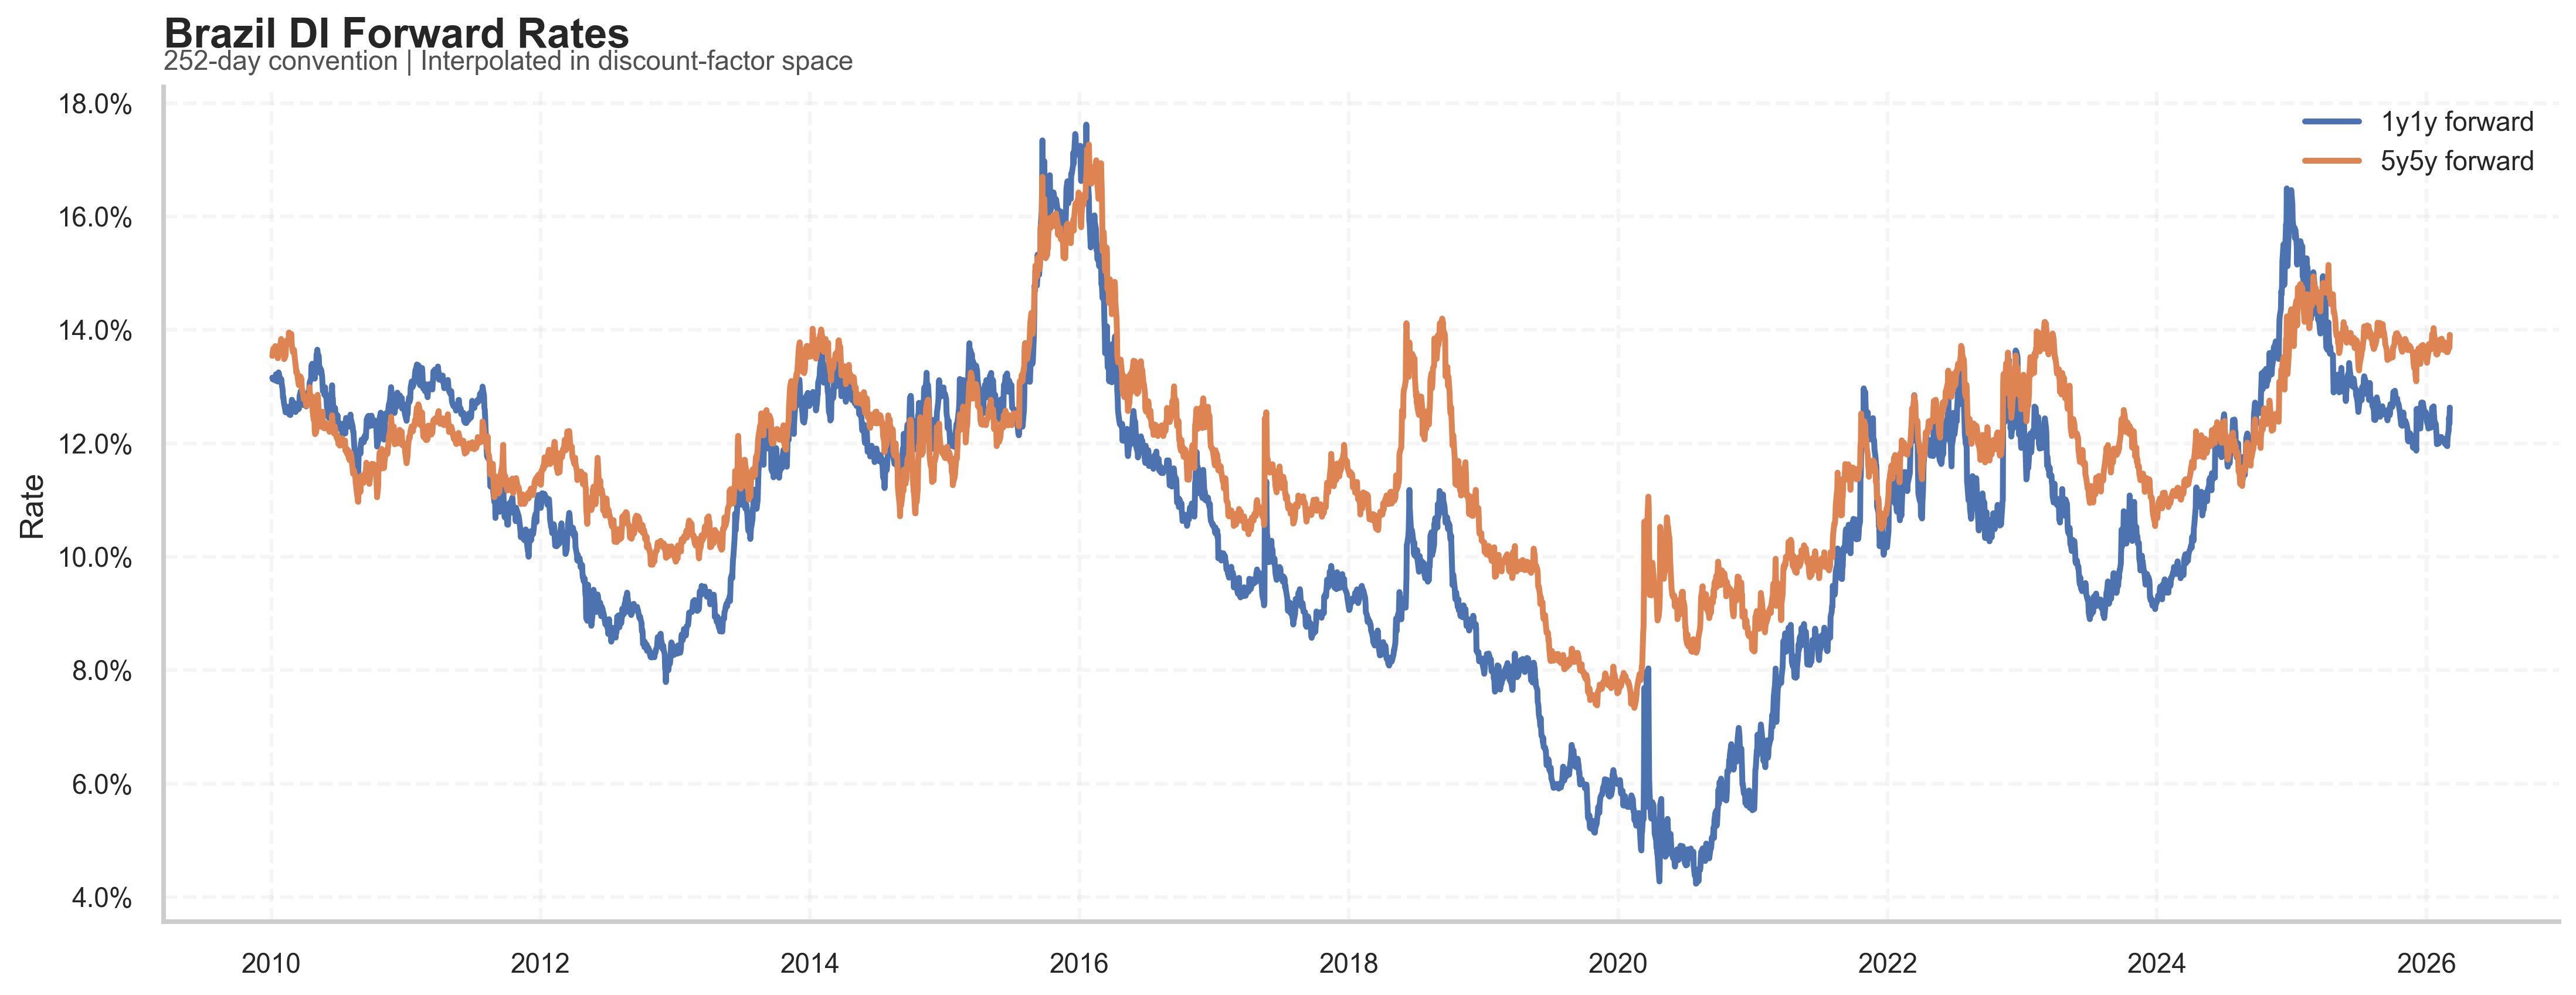
\includegraphics[width=0.92\textwidth]{figures/01_build_DI/fig_01_forwards_1y1y_5y5y_report.png}
	\caption{Constructed Brazil DI forward rates \(1y1y\) and \(5y5y\), obtained from the B3 DI curve through interpolation in discount-factor space.}
	\label{fig:forwards}
\end{figure}
	

	
	\subsection{Target Spread Definition}
	\label{subsec:target_spread}
	
	Having constructed the two forward rates, I define the target variable of the study as the forward slope spread:
	\[
	S_t = 5y5y_t - 1y1y_t.
	\]
	
	This spread captures the relative steepness between a medium-term forward segment and a shorter forward segment of the curve. Economically, \(1y1y\) is more closely related to the nearer-term policy cycle, while \(5y5y\) reflects pricing further ahead in the term structure, where inflation persistence, medium-term policy credibility, and term-premium considerations tend to matter more.
	
	By focusing on \(S_t\), the analysis shifts away from outright rate forecasting and toward a cleaner relative-value object within the curve. This is particularly useful in a macro/rates context, because it reduces the impact of parallel shifts and makes the target more interpretable as a measure of forward slope.
	
	The resulting spread series is shown in Figure \ref{fig:slope_spread}.
	
	\begin{figure}[H]
		\centering
		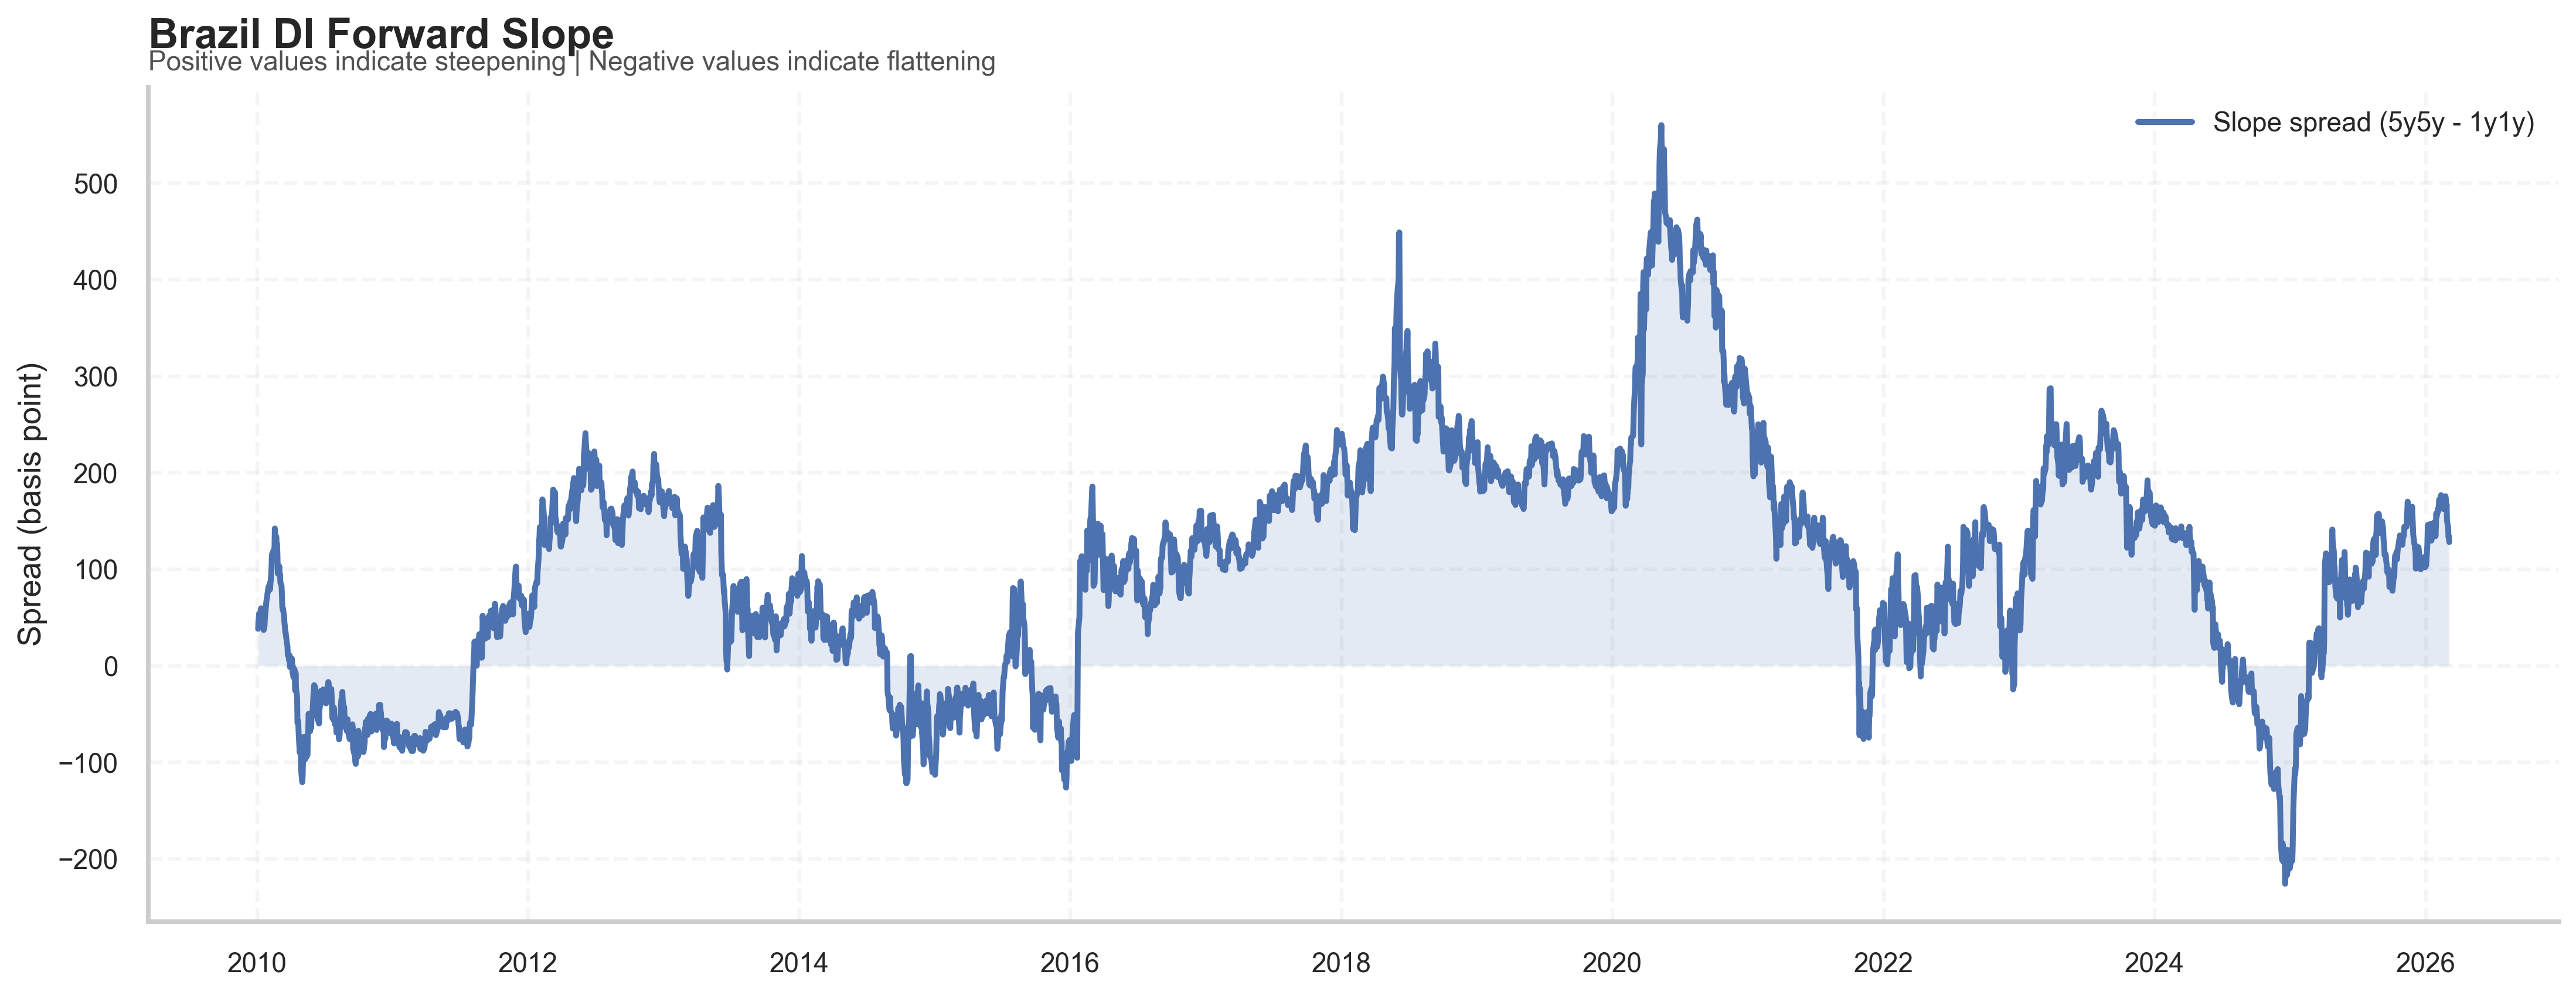
\includegraphics[width=0.92\textwidth]{figures/01_build_DI/fig_02_slope_spread_5y5y_minus_1y1y_report.png}
		\caption{Target spread defined as \(5y5y - 1y1y\). Positive values indicate a steeper forward curve, while lower values indicate relative flattening.}
		\label{fig:slope_spread}
	\end{figure}
	
	With the curve construction and target definition in place, the next step is to investigate whether macroeconomic information helps explain subsequent changes in this forward slope spread.
	
	\section{Macro Data and Hypothesis}
	\label{sec:macro_hypothesis}
	
	\subsection{Macro Inputs}
	\label{subsec:macro_inputs}
	
	Having defined the forward slope spread
	\[
	S_t = 5y5y_t - 1y1y_t,
	\]
	the next step is to investigate whether macroeconomic information helps explain its variation over time.
	
	The macro dataset is intentionally parsimonious and focuses on inflation-related variables, which are the most natural candidates to affect the relative pricing of the Brazilian DI forward curve. In particular, I combine the daily DI spread with three macro series:
	
	\begin{itemize}
		\item monthly IPCA inflation, retrieved from the Central Bank of Brazil's SGS time-series system\footnote{SGS stands for \emph{Time Series Management System}, the public time-series database maintained by the Central Bank of Brazil. In this report, IPCA inflation is taken from SGS series 433, while the seasonally adjusted IBC-Br series is taken from SGS series 24364.};
		\item seasonally adjusted IBC-Br activity data, retrieved from the same SGS database;
		\item 12-month inflation expectations from the BCB Focus survey, using the median forecast.
	\end{itemize}
	
	This choice reflects the economic structure of the Brazilian rates market. The front end of the curve is tightly linked to near-term monetary policy expectations, while the medium-term forward segment is more exposed to inflation persistence, policy credibility, and term-premium effects. For that reason, inflation-related variables are the natural starting point for explaining the dynamics of \(5y5y - 1y1y\).
	
	The emphasis of the analysis is therefore placed on inflation expectations versus realized inflation. IBC-Br is included only as a secondary activity-side control and not as the core driver of the framework.
	
	\subsection{Main Factor Construction}
	\label{subsec:main_factor_construction}
	
	The main macro factor used in the study is the \emph{inflation expectations gap}, defined as:
	\[
	\text{Inflation Expectations Gap}_t
	=
	\text{Focus IPCA 12m}_t - \text{IPCA 12m}_t.
	\]
	
	This variable measures the distance between expected inflation over the next 12 months and recently realized inflation over the previous 12 months. A positive value indicates that expectations are running above realized inflation, which can be interpreted as a sign that inflation persistence is perceived to be rising or, at a minimum, that disinflation is not yet fully credible. A negative value indicates that expectations are below realized inflation, consistent with easing inflation pressure or improving policy credibility.
	
	The appeal of this factor is that it is both economically interpretable and directly connected to the pricing logic of the DI curve. Unlike broader multi-factor approaches, this variable isolates one clear macro mechanism: the interaction between inflation expectations and the inflation actually being observed in the economy.
	
	Figure \ref{fig:main_factor} presents the resulting time series.
	
	\begin{figure}[H]
		\centering
		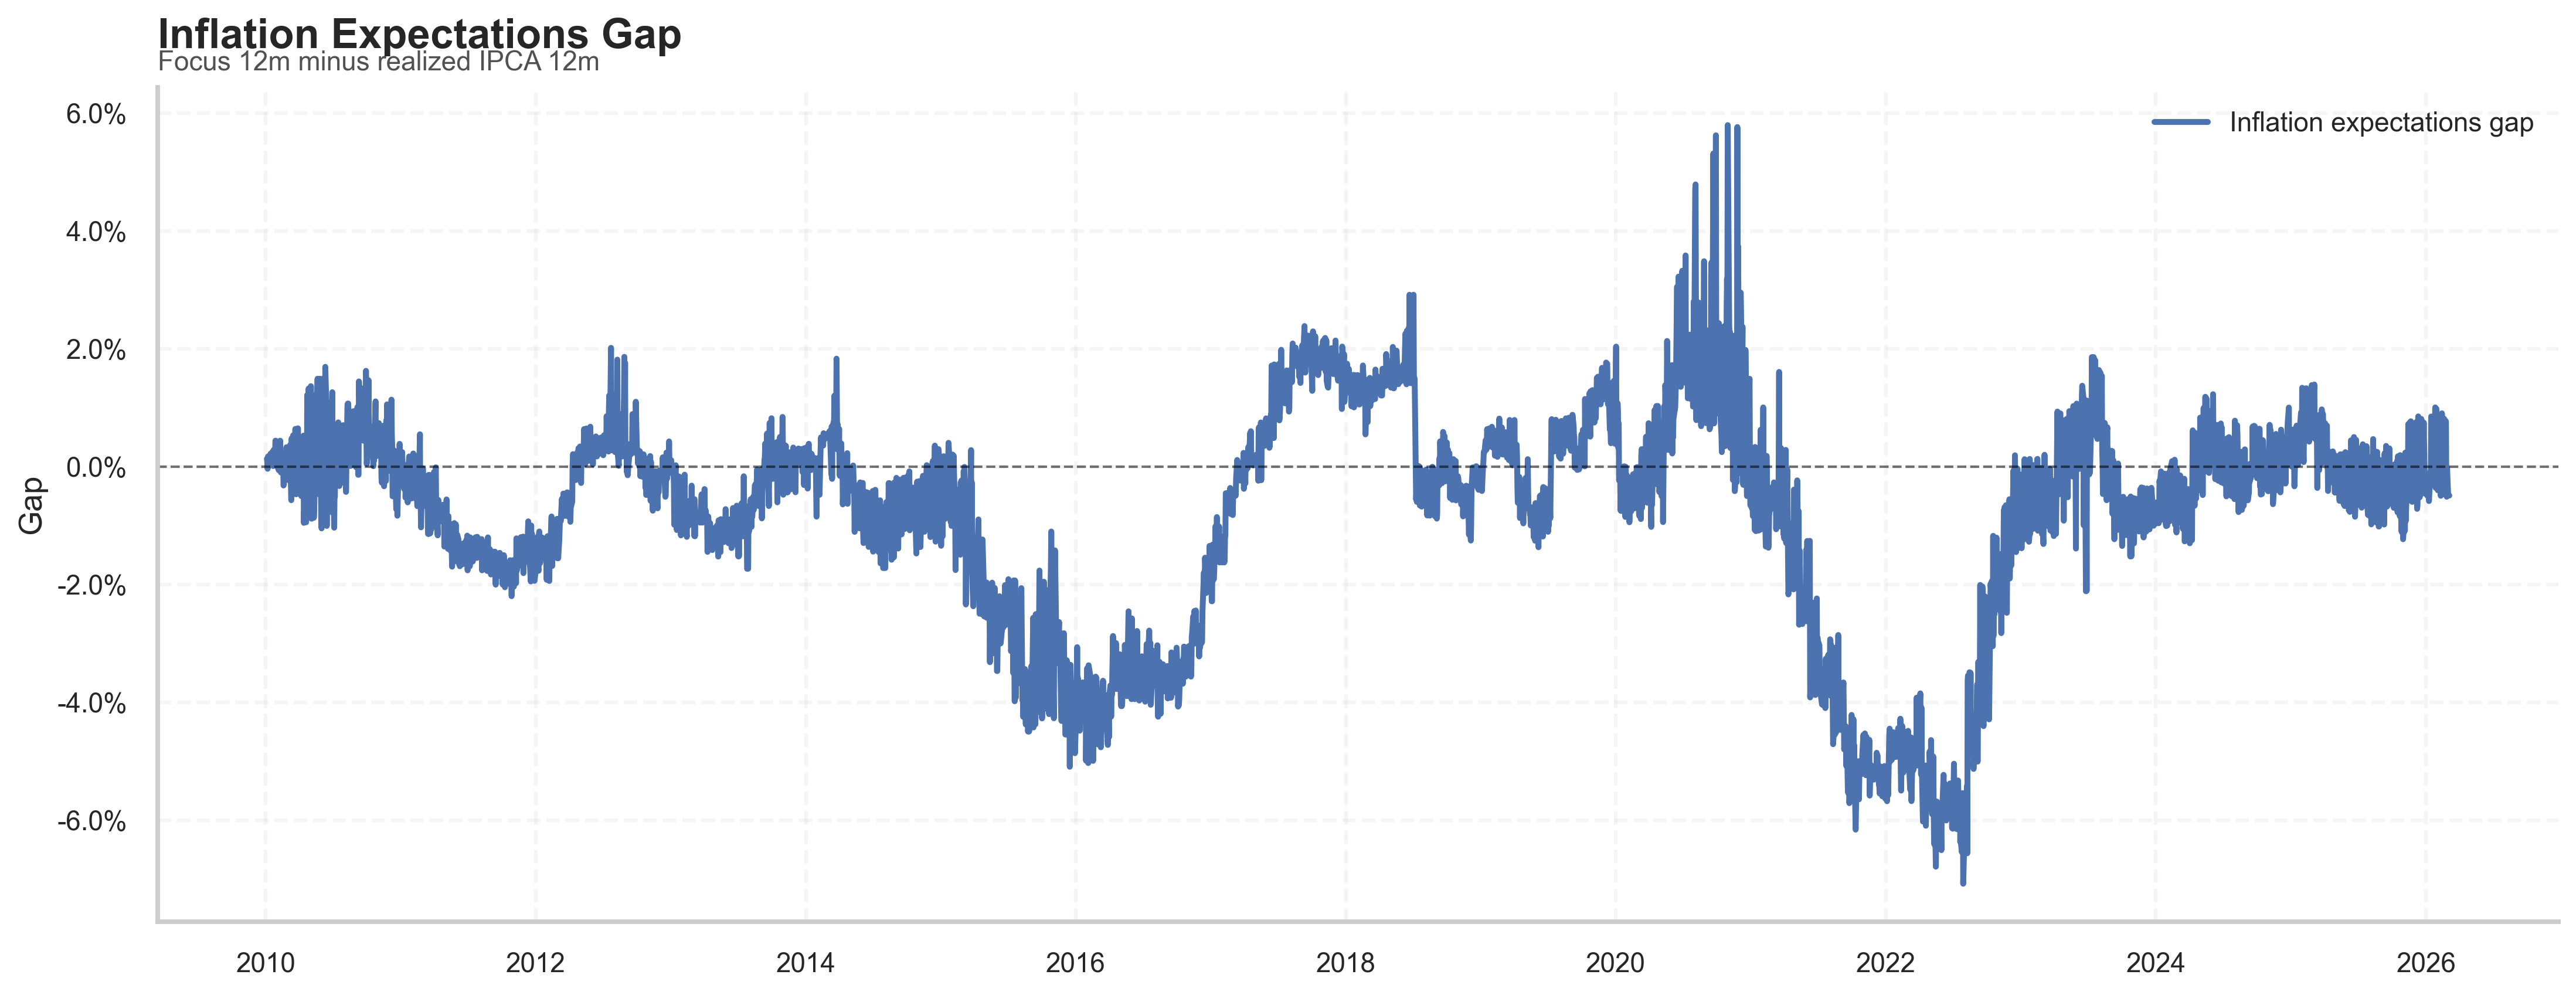
\includegraphics[width=0.92\textwidth]{figures/02_macro/fig_04_inflation_expectations_gap.png}
		\caption{Main macro factor: inflation expectations gap, defined as Focus IPCA 12m minus realized IPCA 12m.}
		\label{fig:main_factor}
	\end{figure}
	
	\subsection{Alternative Inflation Specification}
	\label{subsec:alternative_factor}
	
	As a robustness exercise, I also construct an alternative inflation factor intended to capture shorter-term inflation momentum rather than backward-looking annual inflation:
	\[
	\text{Inflation Persistence Gap}_t
	=
	\text{Focus IPCA 12m}_t - \text{IPCA 3m SAAR}_t.
	\]
	
	Here, the realized inflation leg is replaced by the seasonally adjusted annualized rate implied by the most recent three months of IPCA prints. This alternative specification is useful because annual inflation measures can be slow-moving, whereas short-horizon inflation momentum may better capture turning points in inflation dynamics.
	
	That said, this variable is treated as a secondary robustness measure rather than as the central specification. The reason is that short-term annualized inflation can be noisy and more sensitive to temporary shocks, while the 12-month realized inflation measure provides a cleaner benchmark against which to compare the Focus 12-month expectation.
	
	\subsection{Economic Transmission to the Forward Spread}
	\label{subsec:economic_transmission}
	
	The economic hypothesis of the case is that inflation expectations affect different parts of the DI forward curve asymmetrically.
	
	The \(1y1y\) forward is primarily a policy-horizon measure. It reflects how the market prices the expected stance of monetary policy over the next phase of the cycle and is therefore closely linked to near-term central-bank reaction expectations.
	
	By contrast, the \(5y5y\) forward embeds pricing further ahead in the term structure. At that horizon, the curve is less about the next monetary-policy meetings and more about medium-term inflation persistence, policy credibility, structural risk premium, and the level at which rates are expected to normalize over time. This distinction between a policy-horizon forward and a structural-horizon forward is exactly what makes the spread \(5y5y - 1y1y\) an economically meaningful object to study.
	
	The core hypothesis is therefore:
	
	\begin{quote}
		When inflation expectations move above realized inflation, the market tends to price more inflation persistence and a greater probability that restrictive monetary conditions will remain relevant further ahead in the curve. As a result, the medium-term forward segment should reprice relative to the front-end forward segment, affecting the spread \(5y5y - 1y1y\).
	\end{quote}
	
	In directional terms, the working prior of this report is that a widening inflation expectations gap should, on average, be associated with an increase in the relative steepness of the forward curve as measured by \(5y5y - 1y1y\). The sign and strength of this relationship are then left to the empirical analysis rather than imposed ex ante.
	
	Figure \ref{fig:target_vs_factor} provides a first visual comparison between the target spread and the main macro factor.
	
	\begin{figure}[H]
		\centering
		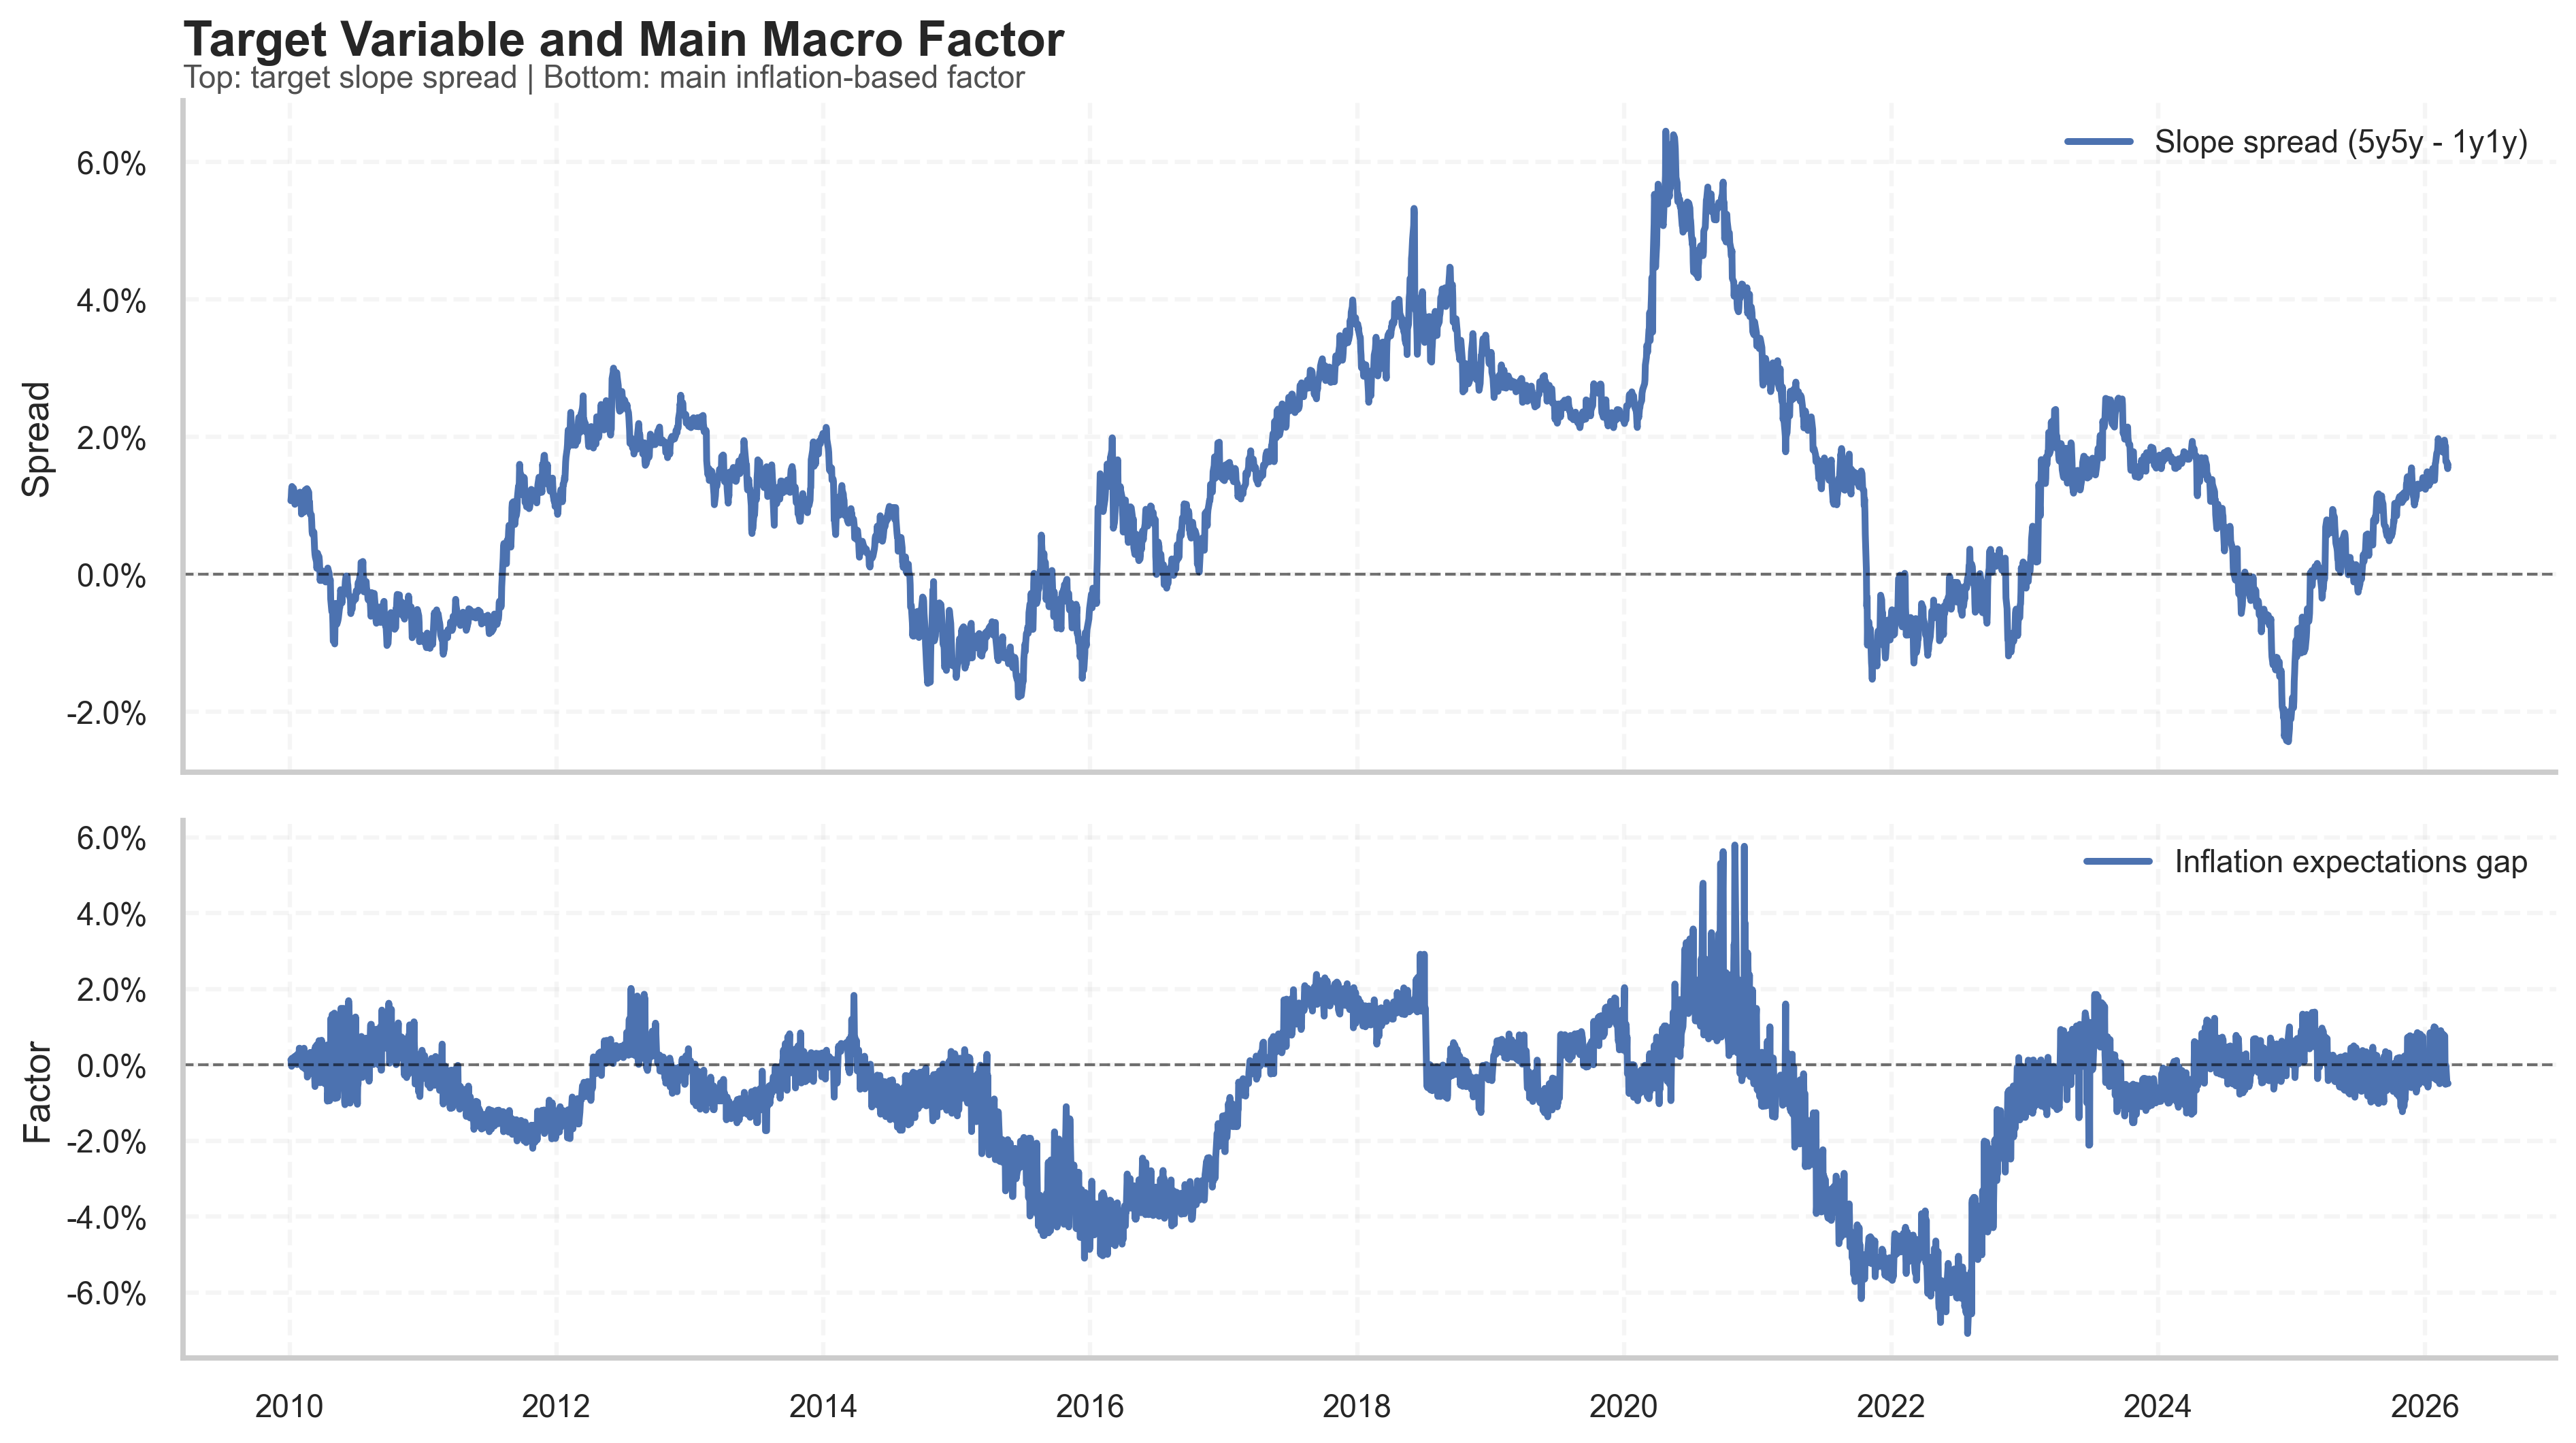
\includegraphics[width=0.92\textwidth]{figures/03_stat_tests/fig_06_target_and_main_factor.png}
		\caption{Visual comparison between the forward slope spread \(5y5y - 1y1y\) and the main macro factor.}
		\label{fig:target_vs_factor}
	\end{figure}
	
	\subsection{Timing and Real-Time Alignment}
	\label{subsec:timing_alignment}
	
	Macro variables are observed at a lower and more discrete frequency than daily DI curve. For this reason, the empirical design aligns each market observation only with information that would have been available in real time. This precaution help prevent look-ahead bias and minimize the risk of overfitting.
	
	\subsection{Role of IBC-Br and Additional Controls}
	\label{subsec:ibc_control}
	
	Although the economic story of the report is centered on inflation, activity conditions may also matter for the forward slope of the DI curve. A stronger-than-expected activity backdrop can reinforce inflation persistence concerns and reduce the market's confidence in future easing, while weaker activity can support disinflation and flatter medium-term pricing.
	
	For this reason, I include seasonally adjusted IBC-Br as a control variable in selected specifications. Its role, however, is intentionally secondary. The central question of the case is not whether a broad macro panel can fit the spread in-sample, but whether a simple and interpretable inflation-related factor contains useful explanatory power for the relative pricing between \(5y5y\) and \(1y1y\).
	
	\subsection{Interpretation for Trading Applications}
	\label{subsec:trading_interpretation}
	
	Even before the formal statistical tests, the macro construction already suggests the right interpretation for implementation.
	
	Because the inflation expectations gap is a relatively slow-moving variable, it is better understood as a macro state variable, regime classifier, or fair-value anchor than as a high-frequency timing signal. In other words, the factor is naturally suited to answer questions such as:
	\begin{itemize}
		\item whether the macro backdrop is more consistent with spread widening or spread compression;
		\item whether the observed forward spread looks rich or cheap relative to the inflation environment;
		\item whether a purely statistical signal should be trusted or filtered given the prevailing inflation regime.
	\end{itemize}
	
	This interpretation is important for the remainder of the case. If the factor proves statistically informative, it can be used either directly in predictive regressions for future spread changes or indirectly as a conditioning variable for a simple trading framework. In both cases, the emphasis remains on economic interpretability rather than on maximizing in-sample fit.
	
	\subsection{What This Section Establishes}
	\label{subsec:macro_section_takeaway}
	
	This section defines a simple but coherent macro hypothesis for the Brazilian DI forward curve. The key idea is that the gap between inflation expectations and realized inflation can help explain the relative pricing of the medium-term and short-term forward segments of the curve.
	
	The next section evaluates that hypothesis formally. In particular, I test whether the inflation expectations gap has predictive content for future changes in the forward slope spread and whether that relationship remains meaningful once simple controls and robustness checks are introduced.
	
	\section{Statistical Validation}
	\label{sec:statistical_validation}
	
	The objective of this section is to evaluate whether the proposed inflation-based macro factor contains useful information for the Brazilian forward slope spread,
	\[
	S_t = 5y5y_t - 1y1y_t,
	\]
	and, more importantly, to determine \emph{how} that information should be interpreted.
	
	This distinction matters. A macro variable can help explain the \emph{level} of a spread without being a strong predictor of its \emph{daily changes}. In the context of the DI curve, this is particularly relevant because inflation-related variables evolve at medium frequency, whereas the spread itself is observed daily and is affected by substantial short-term market noise.
	
	For that reason, the validation is organized in five steps. First, I examine the time-series properties of the target and factor variables. Second, I study lead-lag correlations between the main factor and future spread changes. Third, I estimate predictive regressions across multiple horizons. Fourth, I test whether the factor contributes incremental explanatory power in a lower-frequency Granger framework. Finally, I compare the predictive view with a fair-value view of the spread.
	
	\subsection{Stationarity and Time-Series Properties}
	\label{subsec:stationarity_properties}
	
	Before turning to predictive tests, it is useful to examine the persistence of the spread and macro variables. This matters because forward spreads and macro series often display substantial serial dependence, and regressions in levels can produce misleading inference when persistence is high.
	
	Table \ref{tab:stationarity} reports Augmented Dickey-Fuller (ADF) and KPSS diagnostics for the spread and macro factors, both in levels and in first differences.
	
	\begin{table}[H]
		\centering
		\footnotesize
		\resizebox{\textwidth}{!}{
			\begin{tabular}{lrrrrr}
\toprule
Series & ADF stat & ADF p-value & KPSS stat & KPSS p-value & Obs. \\
\midrule
spread\_level & -2.4064 & 0.1399 & 1.0597 & 0.0100 & 4004 \\
spread\_diff1 & -33.7927 & 0.0000 & 0.0428 & 0.1000 & 4004 \\
main\_factor\_level & -2.4978 & 0.1160 & 0.3029 & 0.1000 & 3977 \\
main\_factor\_diff1 & -10.4981 & 0.0000 & 0.0481 & 0.1000 & 3977 \\
alt\_factor\_level & -6.7739 & 0.0000 & 0.1187 & 0.1000 & 3980 \\
alt\_factor\_diff1 & -8.2015 & 0.0000 & 0.0126 & 0.1000 & 3980 \\
\bottomrule
\end{tabular}

		}
		\caption{Stationarity diagnostics for the target spread and macro factors.}
		\label{tab:stationarity}
	\end{table}
	
The results suggest that the spread level is strongly persistent. For \texttt{spread\_level}, the ADF test does not reject a unit root at conventional significance levels, while the KPSS test rejects level stationarity. By contrast, \texttt{spread\_diff1} appears clearly stationary under both diagnostics. This indicates that the level of the forward-slope spread is not well treated as a stable mean-reverting series over the full sample, whereas its short-run changes are much better behaved statistically.

The main macro factor shows a similar but slightly more nuanced pattern. In levels, the ADF result does not reject a unit root, while the KPSS result does not reject stationarity. Rather than reading this as definitive evidence in either direction, the more cautious interpretation is that the main factor is highly persistent in levels and becomes considerably more regular once transformed into first differences. This is economically plausible, since inflation-expectation misalignment is a slow-moving macro variable rather than a high-frequency market signal.

The alternative inflation-persistence factor is statistically better behaved in levels, with stronger evidence of stationarity in the table. However, this cleaner time-series profile comes with a trade-off: because it is constructed from shorter-horizon inflation dynamics, it is also more exposed to temporary inflation noise and may be less economically stable as a medium-frequency state variable.

These diagnostics guide the empirical design of the next subsections. The predictive exercises are therefore run on future changes in the spread rather than on the raw spread level, and inference is made robust to serial dependence and overlapping forecast horizons. More broadly, the stationarity results already suggest an important theme of the case: the macro factor is more naturally interpreted as a medium-frequency valuation anchor than as a daily timing signal..
	
	\subsection{Lead-Lag Correlation Evidence}
	\label{subsec:lead_lag_evidence}
	
	As a preliminary diagnostic, I examine lagged correlations between the main macro factor and future changes in the forward-slope spread:
	
	\[
	\Delta_h S_{t+h} = S_{t+h} - S_t,
	\]
	for forecast horizons \(h \in \{5, 21, 63\}\) business days.
	
	Figure \ref{fig:lagged_corr} summarizes the correlation profiles. The evidence is weak at short horizons. At the 5-day horizon, correlations are essentially zero across lags, suggesting that the macro factor does not contain meaningful information for very short-term spread timing. At the 21-day horizon, correlations remain small and mostly negative, still without a strong or economically decisive pattern.
	
	\begin{figure}[H]
		\centering
		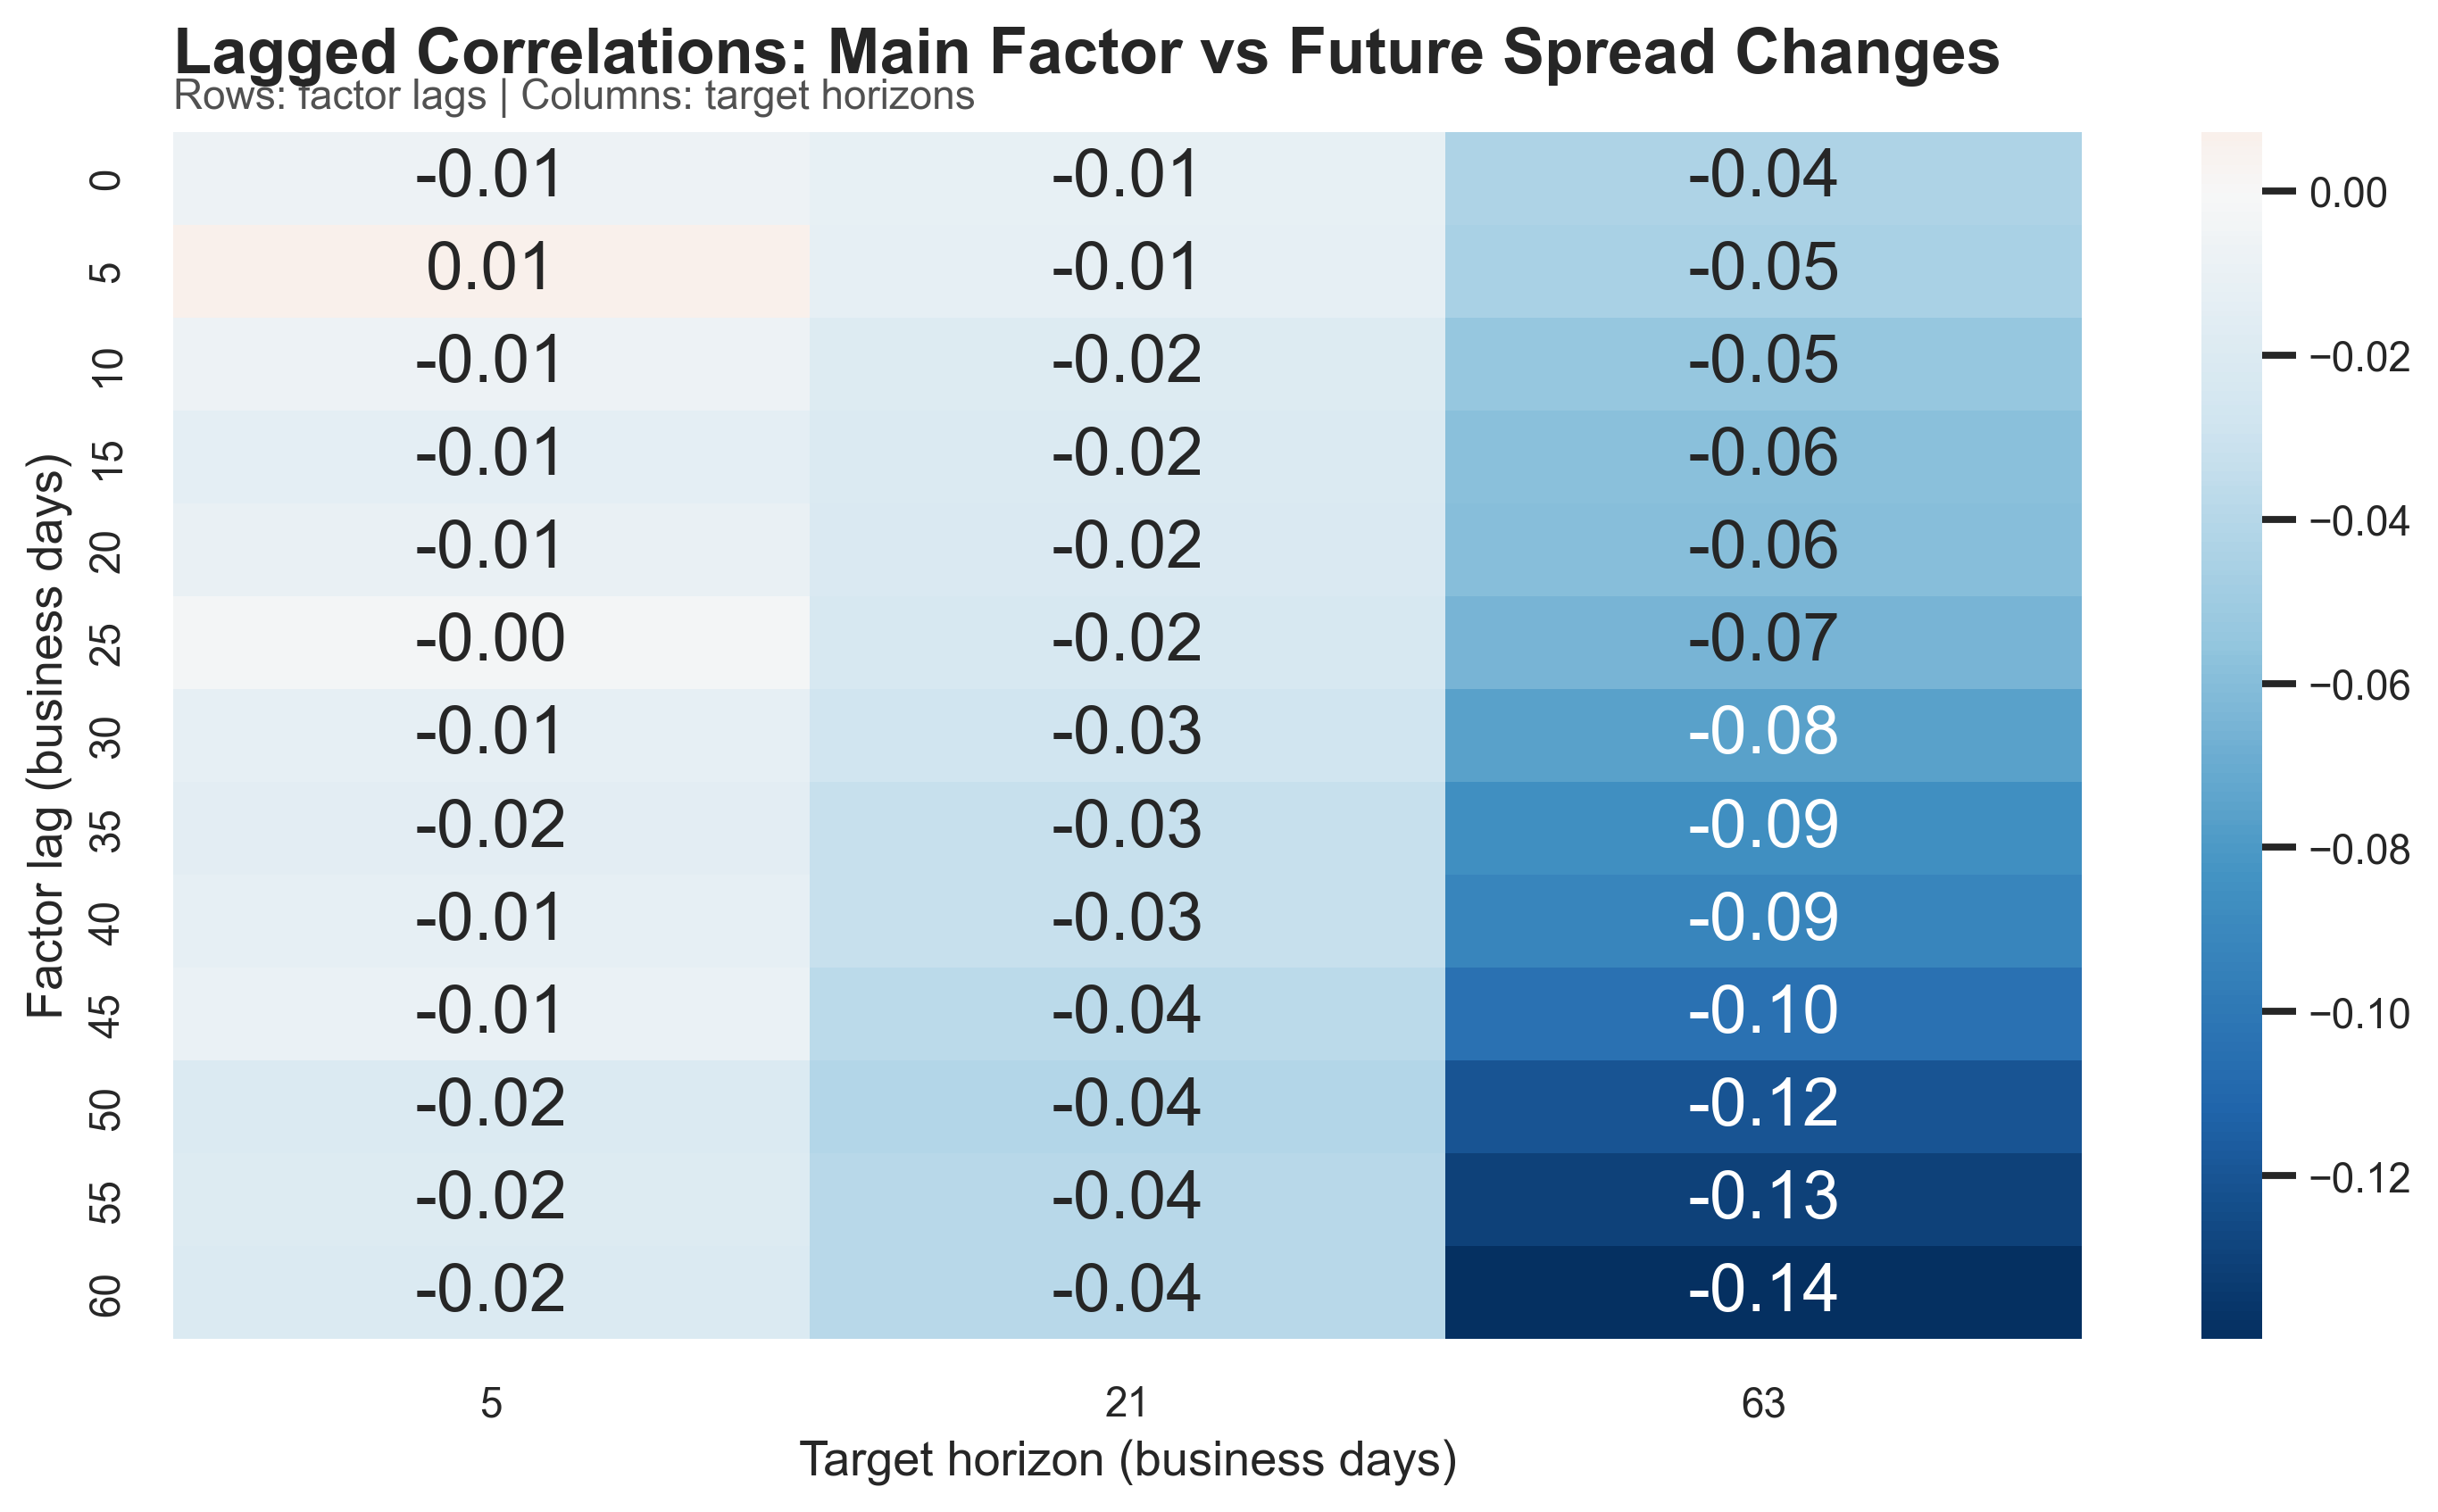
\includegraphics[width=0.92\textwidth]{figures/03_stat_tests/fig_07_lagged_correlation_heatmap_main.png}
		\caption{Lagged correlations between the main macro factor and future spread changes across forecast horizons.}
		\label{fig:lagged_corr}
	\end{figure}
	
	A more visible structure appears only at the 63-day horizon. In that case, correlations become more negative as the factor is lagged further, with somewhat larger absolute values at longer lags. Even so, the magnitudes remain moderate, so the result should be interpreted cautiously. Rather than indicating a strong directional forecasting signal, the evidence suggests only that the macro factor may contain some medium-frequency information about subsequent spread adjustment.
	
	This interpretation is consistent with the economic nature of the factor. The inflation expectations gap is a slow-moving macro variable, whereas the forward spread is observed daily and is influenced by substantial short-run market noise. For that reason, it is not surprising that the relationship is weak at short horizons and only becomes faintly visible over longer windows.
	
	Overall, the lead-lag evidence supports a restrained conclusion: the main macro factor does not behave like a short-horizon trading signal, but it may still carry medium-frequency information that is more relevant for valuation or regime interpretation than for daily forecasting.
	
	\subsection{Predictive Regressions}
	\label{subsec:predictive_regressions}
	
	I next estimate predictive regressions of the form
	\[
	\Delta_h S_{t+h}
	=
	\alpha_h + \beta_h Z(M_t) + \varepsilon_{t+h},
	\]
	where \(Z(M_t)\) is the standardized macro factor and \(h\) is the forecast horizon.
	
	Because the dependent variables overlap for horizons beyond one day, I estimate all regressions with HAC (Newey-West) standard errors. This is essential to avoid overstating significance.
	Table \ref{tab:pred_regs} reports the univariate predictive results for the two inflation-based factors, and Figure \ref{fig:beta_horizons} summarizes the estimated betas by horizon.
	
	\begin{table}[H]
		\centering
		\footnotesize
		\resizebox{\textwidth}{!}{
			\begin{tabular}{llrrrrrrr}
\toprule
Factor & Standardized factor & Horizon (days) & Obs. & Alpha & Beta & t-stat & p-value & R-squared \\
\midrule
Inflation expectations gap & Inflation expectations gap (z) & 5 & 4004 & 0.0005 & -0.0022 & -0.2253 & 0.8217 & 0.0001 \\
Inflation expectations gap & Inflation expectations gap (z) & 21 & 3988 & 0.0035 & -0.0065 & -0.1742 & 0.8617 & 0.0001 \\
Inflation expectations gap & Inflation expectations gap (z) & 63 & 3946 & 0.0116 & -0.0401 & -0.4626 & 0.6436 & 0.0019 \\
Inflation persistence gap & Inflation persistence gap (z) & 5 & 4004 & 0.0005 & 0.0027 & 0.2813 & 0.7785 & 0.0001 \\
Inflation persistence gap & Inflation persistence gap (z) & 21 & 3988 & 0.0036 & 0.0132 & 0.3921 & 0.6950 & 0.0006 \\
Inflation persistence gap & Inflation persistence gap (z) & 63 & 3946 & 0.0128 & 0.0781 & 1.1241 & 0.2610 & 0.0071 \\
\bottomrule
\end{tabular}

		}
		\caption{Predictive regressions of future spread changes on inflation-based macro factors.}
		\label{tab:pred_regs}
	\end{table}
	
	\begin{figure}[H]
		\centering
		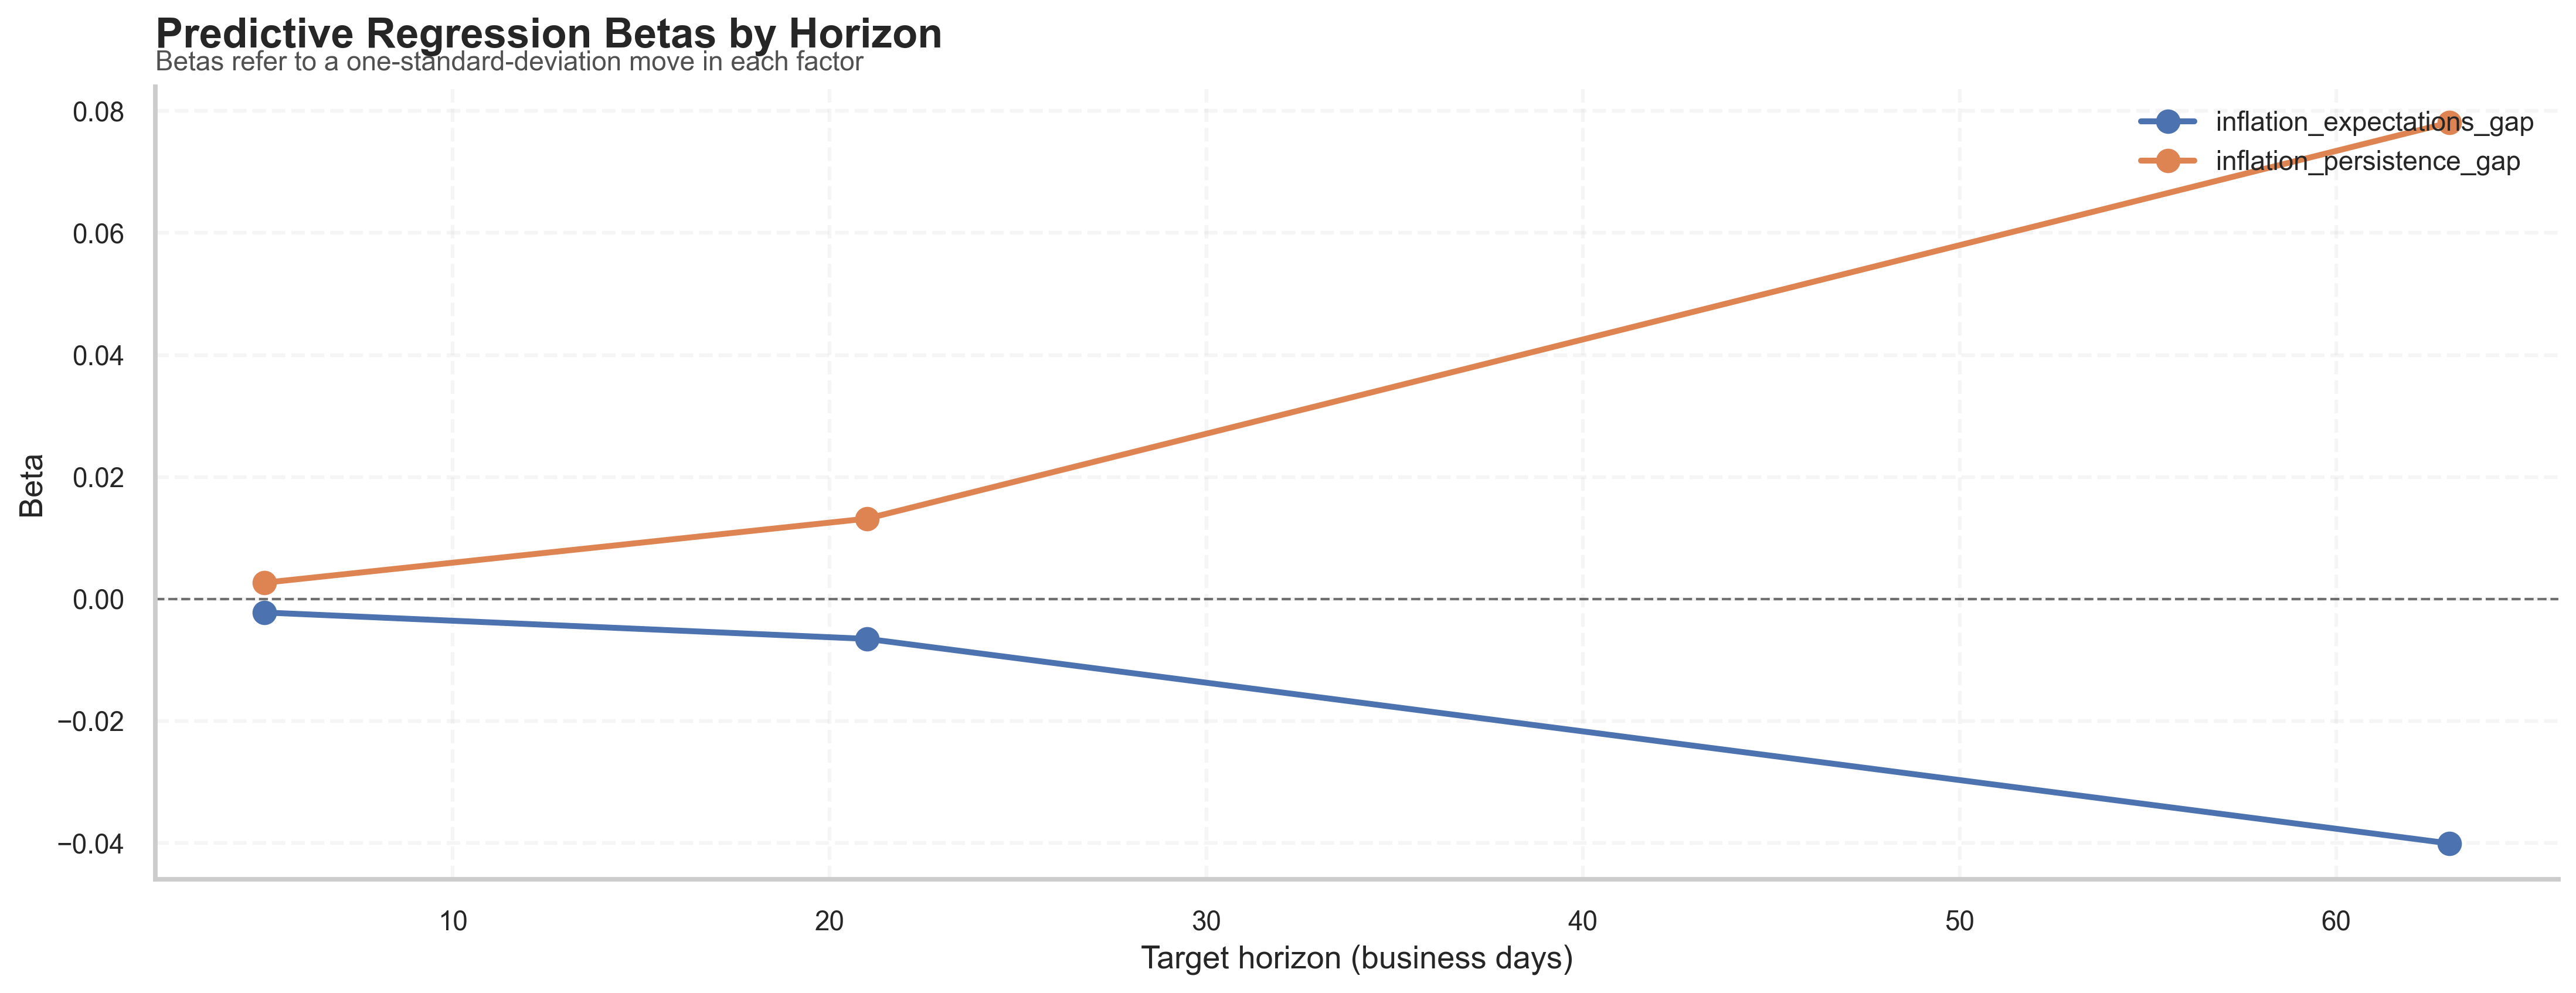
\includegraphics[width=0.92\textwidth]{figures/03_stat_tests/fig_08_predictive_betas_by_horizon.png}
		\caption{Predictive regression betas by horizon for the main and alternative inflation factors.}
		\label{fig:beta_horizons}
	\end{figure}
	
	The results are intentionally interpreted conservatively. For the main factor, the estimated betas are small and negative at all horizons, with very low explanatory power and no statistical significance. The point estimates become somewhat larger in magnitude at the 63-day horizon, but remain far from decisive.
	
	The alternative inflation persistence factor performs somewhat better empirically, especially at the longest horizon, where the beta increases in magnitude. Still, the explanatory power remains low and the statistical evidence is not strong enough to support a robust standalone directional claim.
	
	This is one of the most important findings of the report. The economic hypothesis is coherent, but in the strict formulation of \emph{predicting daily future spread changes}, the inflation factors are weak. This does not invalidate the macro intuition; rather, it suggests that the information content of the factor is not best expressed as a short-horizon forecasting signal.
	
	\subsection{Predictive Regressions with an IBC-Br Control}
	\label{subsec:predictive_with_control}
	
	To assess whether the inflation factor retains incremental predictive content once a simple activity proxy is included, I augment the baseline predictive regression with the seasonally adjusted IBC-Br series. The goal is to test whether the inflation-based signal survives after controlling for a secondary macro variable linked to the activity side of the economy.
	
	The equation is:
	
	\[
	\Delta_h S_{t+h} = \alpha_h + \beta_h Z(M_t) + \gamma_h Z(IBCBr_t) + \varepsilon_{t+h},
	\]
	
	where \(\Delta_h S_{t+h} = S_{t+h} - S_t\) is the future change in the forward-slope spread over horizon \(h\), \(Z(M_t)\) is the standardized main inflation factor, and \(Z(IBCBr_t)\) is the standardized IBC-Br control. As in the previous subsection, inference is based on HAC (Newey--West) standard errors because the forecast-horizon dependent variables overlap across observations.
	
	\begin{table}[H]
		\centering
		\footnotesize
		\resizebox{\textwidth}{!}{
			\begin{tabular}{rrrrrrr}
\toprule
Horizon (days) & Obs. & Beta (main factor) & t-stat (main factor) & Beta (control) & t-stat (control) & R-squared \\
\midrule
5 & 4004 & -0.0025 & -0.2507 & 0.0043 & 0.4975 & 0.0003 \\
21 & 3988 & -0.0077 & -0.2073 & 0.0219 & 0.6902 & 0.0017 \\
63 & 3946 & -0.0423 & -0.4946 & 0.0495 & 0.5790 & 0.0045 \\
\bottomrule
\end{tabular}

		}
		\caption{Predictive regressions including an activity-side control.}
		\label{tab:pred_regs_control}
	\end{table}
	
	The Table \ref{tab:pred_regs_control} reports the results. The addition of the IBC-Br control does not materially improve the predictive performance of the regression. The coefficient on the main factor remains small and statistically weak across horizons, while the coefficient on IBC-Br is also not statistically strong. The overall explanatory power remains very low.
	
	This result suggests that the weakness of the predictive regressions is not simply due to the omission of a basic activity-side control. More broadly, it reinforces the idea that medium-frequency macro variables, whether inflation-based or activity-based, struggle to explain noisy daily changes in the spread in an unconditional linear specification. In that sense, the main inflation factor appears to contain limited short-horizon forecasting power even after conditioning on a simple macro control.
	

	
	\subsection{Granger-Causality Diagnostics}
	\label{subsec:granger_diagnostics}
	
	As an additional check on temporal ordering, I run Granger-causality tests using lower-frequency transformations of the series.
	
	\begin{table}[H]
		\centering
		\footnotesize
		\resizebox{\textwidth}{!}{
			\begin{tabular}{lrr}
\toprule
Factor & Lag (weeks) & p-value \\
\midrule
Inflation expectations gap & 1 & 0.4042 \\
Inflation expectations gap & 2 & 0.4839 \\
Inflation expectations gap & 3 & 0.6060 \\
Inflation expectations gap & 4 & 0.6563 \\
Inflation persistence gap & 1 & 0.4885 \\
Inflation persistence gap & 2 & 0.7910 \\
Inflation persistence gap & 3 & 0.4841 \\
Inflation persistence gap & 4 & 0.1831 \\
\bottomrule
\end{tabular}

		}
		\caption{Weekly Granger-causality diagnostics for the inflation-based macro factors.}
		\label{tab:granger}
	\end{table}
	
	The p-values do not provide strong evidence that either inflation factor Granger-causes future spread changes in this specification. This result is consistent with the predictive regressions: whatever macro information exists is not strong enough to dominate the short- to medium-horizon statistical variation of the spread in a simple linear forecasting setup.
	
	These tests should be interpreted cautiously. Granger causality is not economic causality, and failure to reject the null does not imply that the macro hypothesis is wrong. Instead, it suggests that the informational channel is weaker, slower, and more regime-dependent than a linear predictive test is able to capture.
	
	\subsection{Parameter Stability and Regime Dependence}
	\label{subsec:parameter_stability}
	
	A key question for implementation is whether the relationship between the main macro factor and future spread changes is stable over time. To assess that, I estimate rolling predictive regressions for the 21-day horizon.
	
	\[
	\Delta_{21} S_{t+21} = \alpha_{\tau} + \beta_{\tau} Z(M_t) + \varepsilon_{t+21},
	\qquad t \in \mathcal{W}_{\tau},
	\]
	
	where \(\mathcal{W}_{\tau}\) denotes rolling estimation window \(\tau\). I then track the estimated \(\beta_{\tau}\) and its associated t-statistic across windows.
	
	\begin{figure}[H]
		\centering
		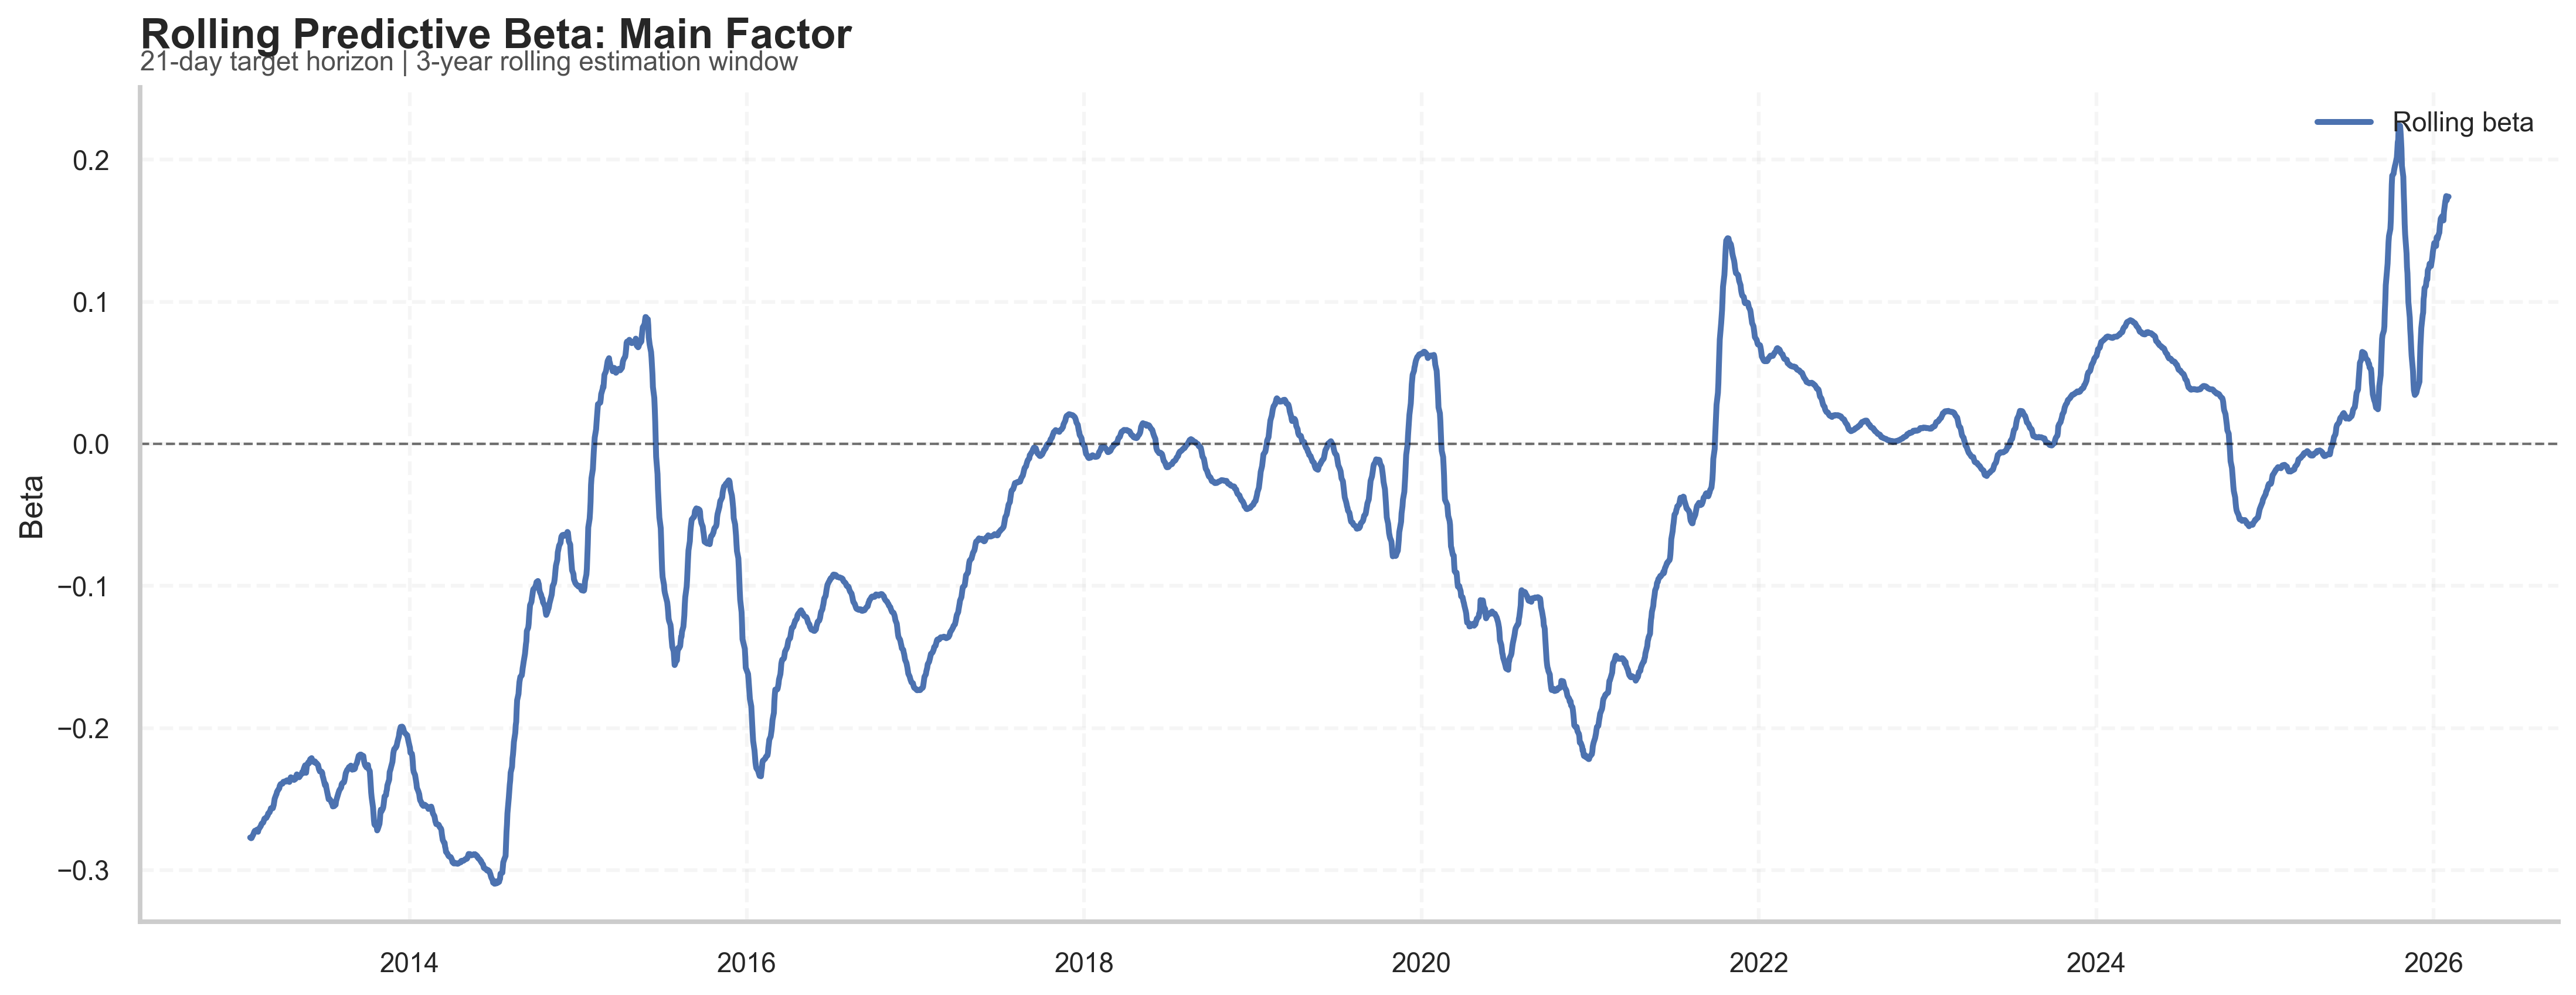
\includegraphics[width=0.92\textwidth]{figures/03_stat_tests/fig_09_rolling_beta_main_factor.png}
		\caption{Rolling predictive beta of the main macro factor for 21-day future spread changes.}
		\label{fig:rolling_beta}
	\end{figure}
	
	\begin{figure}[H]
		\centering
		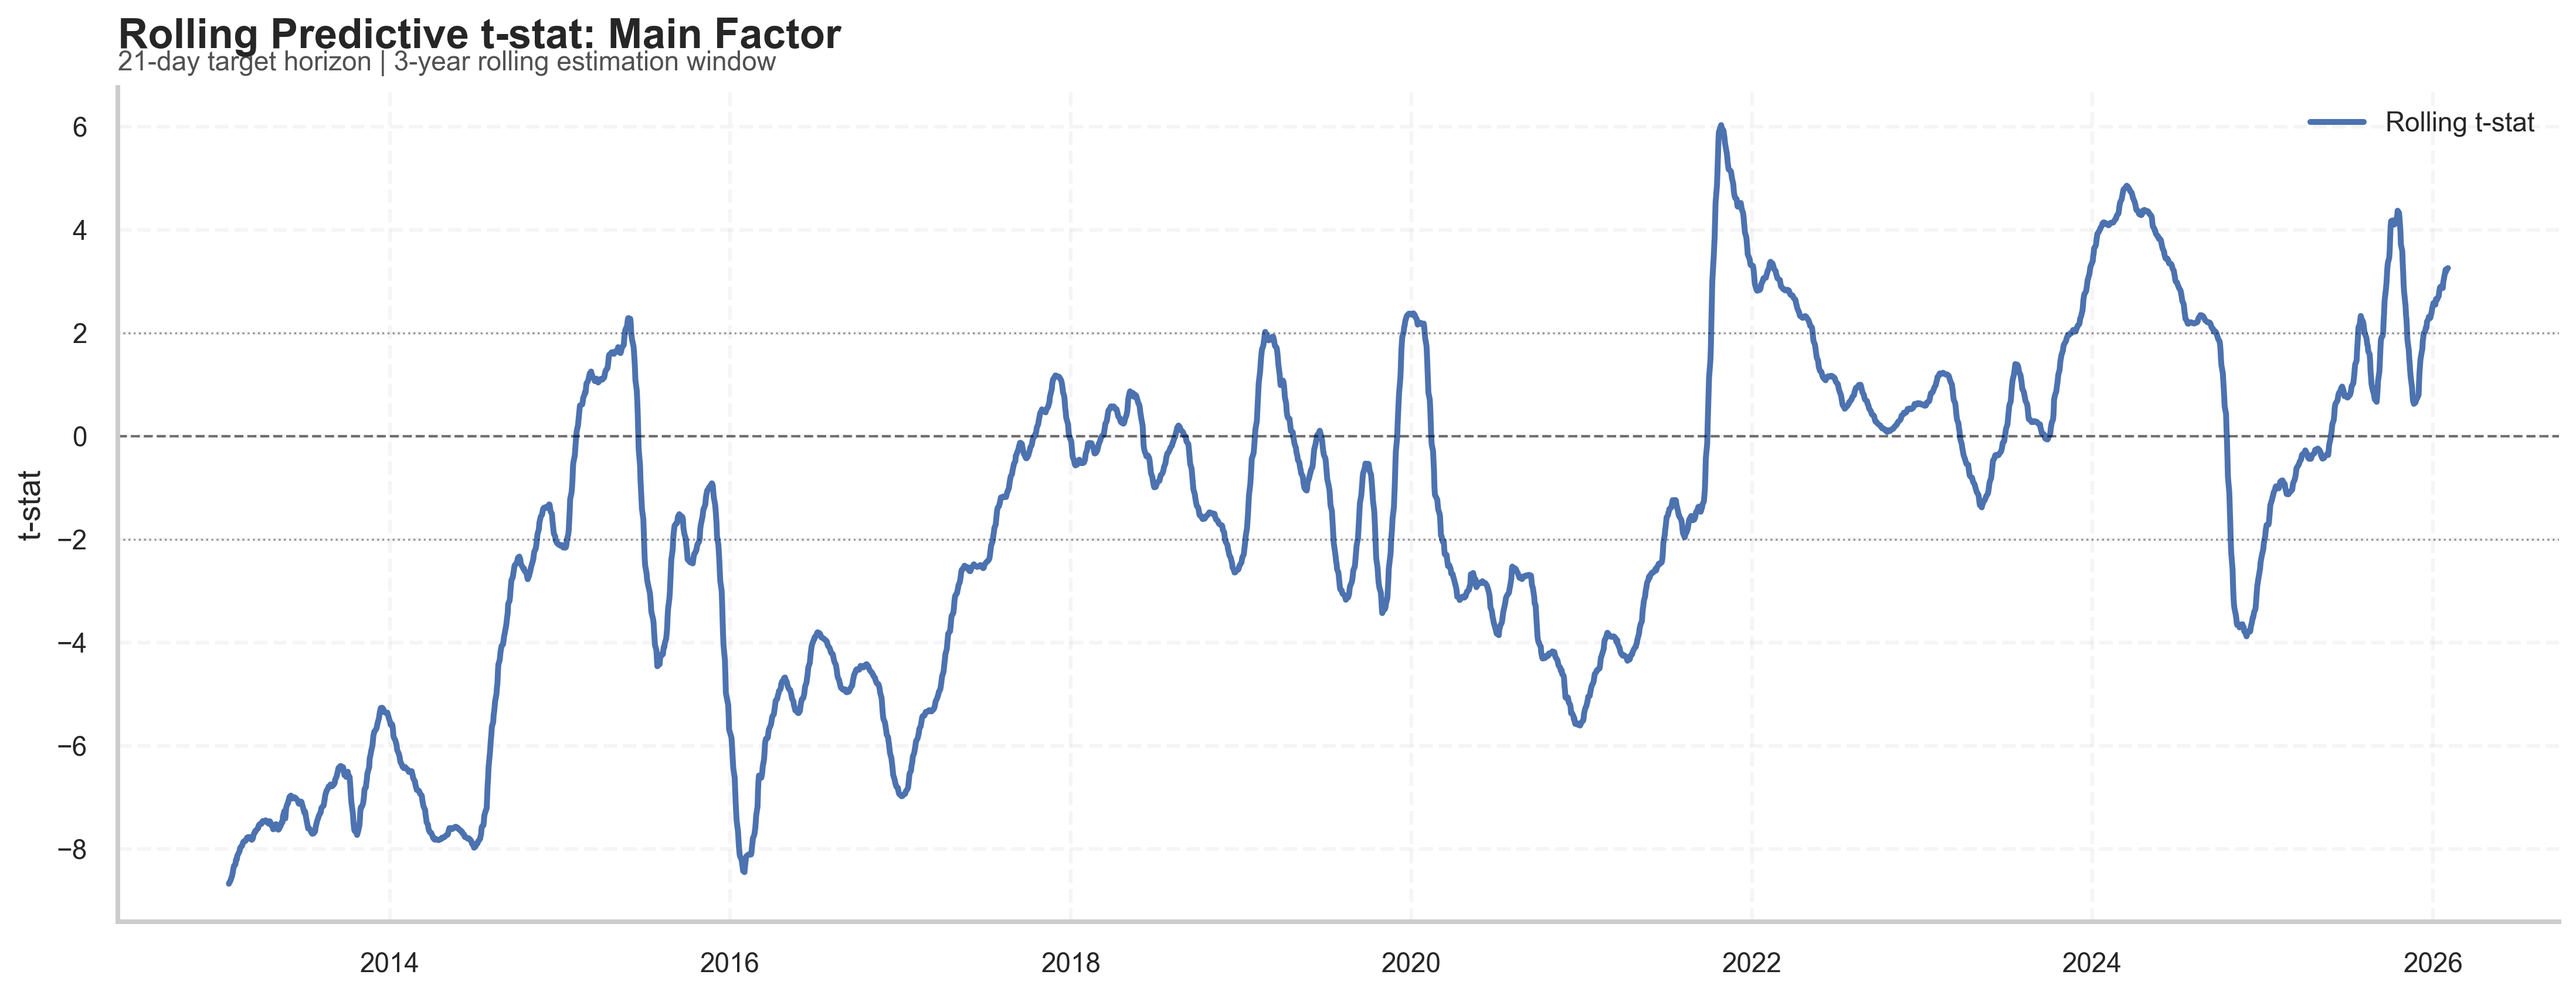
\includegraphics[width=0.92\textwidth]{figures/03_stat_tests/fig_10_rolling_tstat_main_factor.png}
		\caption{Rolling predictive t-statistic of the main macro factor for 21-day future spread changes.}
		\label{fig:rolling_tstat}
	\end{figure}
	
	The rolling analysis shows substantial instability. Both the sign and magnitude of the coefficient vary meaningfully across subperiods, and the corresponding t-statistic frequently crosses zero. In some windows the relationship appears strongly negative, while in others it weakens materially or even changes sign.
	
	Economically, this is plausible. The relevance of an inflation expectations gap for the DI curve depends on the broader macro regime: inflation-target credibility, policy uncertainty, fiscal backdrop, external rates pressure, and the degree to which the front end or the longer end is driving the repricing. A single stable coefficient is therefore unlikely to summarize the full sample well.
	
	This instability is a central reason why the factor should not be treated as a static unconditional alpha source.
	
	\subsection{A Fair-Value Interpretation}
	\label{subsec:fair_value_interpretation}
	
	Although the main inflation factor is weak in forecasting future spread changes, it performs materially better in a fair-value specification for the level of the spread. This is consistent with the broader interpretation developed earlier in the report: macro variables may be more informative about where a relative-value spread should trade than about its short-horizon day-to-day movements. In the DI curve, this distinction is especially relevant because inflation-related variables evolve at medium frequency, whereas the spread itself is observed daily and is affected by substantial short-term market noise.
	
	I therefore also estimate regressions of the form
	\[
	S_t = \alpha + \beta M_t + u_t,
	\]
	and
	\[
	S_t = \alpha + \beta_1 M_t + \beta_2 X_t + u_t,
	\]
	where  \(S_t\) is the forward-slope spread, \(M_t\) is the main inflation factor and \(X_t\) is a simple macro control.
	
	\begin{table}[H]
		\centering
		\footnotesize
		\resizebox{\textwidth}{!}{
			\begin{tabular}{lrrrrrr}
\toprule
Specification & Obs. & R-squared & Beta (main factor) & t-stat (main factor) & Beta (control) & t-stat (control) \\
\midrule
Main factor only & 4009 & 0.2281 & 0.7649 & 9.3362 &  &  \\
Main factor + activity control & 4009 & 0.4044 & 0.8039 & 12.4879 & -0.6735 & -8.0678 \\
\bottomrule
\end{tabular}

		}
		\caption{Fair-value regressions for the spread level.}
		\label{tab:fair_value_regs}
	\end{table}
	

	
	Table \ref{tab:fair_value_regs} reports the results. The fair-value regressions are materially stronger than the predictive-change regressions. In the univariate specification, the main factor explains a meaningful fraction of the variation in the spread level. Adding the control variable increases the fit further, indicating that the level of the spread is more closely related to the macro backdrop than the earlier short-horizon forecasting exercises suggested.
	
	The interpretation of this result should remain measured. It does not imply that the model fully determines market pricing, nor that the estimated fair value is exact. Rather, it suggests that the inflation expectations gap is more useful as a medium-frequency anchor for the level of the spread than as a precise predictor of near-term spread changes.
	
	This naturally supports a relative-value interpretation of the framework. Instead of trading the macro factor directionally in isolation, a more coherent implementation is to estimate a macro-implied fair value for the spread and then evaluate whether market pricing is rich or cheap relative to that benchmark.
	
	\subsection{Summary of Statistical Evidence}
	\label{subsec:summary_statistical_evidence}
	
	Taken together, the statistical evidence leads to a nuanced but coherent conclusion.
	
	First, the macro hypothesis is economically plausible and the data construction is internally consistent. Second, the inflation expectations gap does \emph{not} emerge as a strong standalone predictor of future daily spread changes; lagged correlations are weak, predictive regressions have low explanatory power, and Granger tests do not provide strong support. Third, the rolling analysis shows that any predictive relationship is unstable and highly regime-dependent.
	
	At the same time, the factor is far more useful in a fair-value interpretation of the spread level. This suggests that the right role for the macro factor is not as a pure short-horizon alpha signal, but as a medium-frequency state variable, regime classifier, or macro valuation anchor.
	
	This conclusion is important for the implementation stage. The next section therefore does not treat the macro factor as an unconditional forecasting engine. Instead, it uses the statistical evidence to motivate a simple trading framework in which macro information conditions or anchors trading decisions rather than fully determining them.
	
	\section{Trading Framework and Backtest}
	\label{sec:trading_backtest}
	
	\subsection{From Macro Factor to Trading Signal}
	\label{subsec:macro_to_signal}
	
	The statistical analysis suggests that the inflation-based macro factor is weak as a standalone predictor of short-horizon daily changes in the forward slope spread. However, the same factor is more informative when interpreted as a macro anchor for the \emph{level} of the spread.
	
	For that reason, the trading framework is built around a fair-value formulation rather than a direct directional forecast. At each date \(t\), I estimate a macro-implied fair value for the target spread
	\[
	S_t = 5y5y_t - 1y1y_t
	\]
	using a walk-forward regression based only on information available up to that date. The baseline specification is:
	\[
	S_t = \alpha_t + \beta_t Z(M_t) + \varepsilon_t,
	\]
	where \(M_t\) is the main macro factor and \(Z(M_t)\) denotes its standardized value relative to the trailing estimation window. In some robustness checks, I also include a simple activity-side control.
	
	The fitted value from this regression defines the model-implied fair value of the spread,
	\[
	\widehat{S}^{\text{fair}}_t.
	\]
	
	I then define mispricing as the deviation between fair value and the observed spread:
	\[
	\text{mispricing}_t = \widehat{S}^{\text{fair}}_t - S_t.
	\]
	
	A positive mispricing indicates that the observed spread is below the level suggested by the macro backdrop, which is interpreted as a relative flattening versus fair value and therefore as a potential steepener opportunity. A negative mispricing indicates that the observed spread is above macro-implied fair value and is therefore interpreted as a potential flattener opportunity.
	
	\subsection{Signal Standardization and Position Rules}
	\label{subsec:signal_rules}
	
	Because the raw mispricing series is persistent and time-varying in scale, I standardize it using a rolling z-score computed out-of-sample:
	\[
	z_t =
	\frac{\text{mispricing}_t - \mu_t}{\sigma_t},
	\]
	where \(\mu_t\) and \(\sigma_t\) are estimated using only backward-looking information from a rolling window.
	
	The strategy activates positions only when the deviation from fair value becomes sufficiently large in standardized terms. In the baseline implementation, the position rule is symmetric:
	
	\begin{itemize}
		\item enter a long spread position when \(z_t \geq z^{entry}\),
		\item enter a short spread position when \(z_t \leq -z^{entry}\),
		\item exit an existing position once the z-score reverts toward zero below an exit threshold.
	\end{itemize}
	
	This rule is intentionally simple. The objective is not to optimize entry and exit in-sample, but to test whether macro-implied valuation dislocations in the spread tend to normalize often enough to support a usable relative-value framework.
	
	\subsection{Backtest Design}
	\label{subsec:backtest_design}
	
	The backtest is implemented in a walk-forward manner. At each date, the fair-value model is estimated only on trailing data, and both the signal construction and position decisions use only information available in real time. This ensures consistency with the no-look-ahead discipline imposed in the macro-data construction stage.
	
	Position sizing is expressed in stylized spread-DV01 terms. The baseline implementation assumes a constant spread exposure corresponding to a DV01 of 10,000 per basis point of spread move whenever a full unit position is active. This makes the PnL interpretable in economic terms while keeping the implementation transparent.
	
	Daily gross PnL is computed from the lagged position multiplied by the next-day change in the spread, expressed in basis points. Transaction costs are modeled as a fixed cost per unit of turnover. The backtest is therefore intended as a \emph{stylized spread-level implementation}, not as a full instrument-level strategy with explicit contract selection, exact hedge ratios, or execution microstructure.
	
	\subsection{PnL Decomposition}
	\label{subsec:pnl_decomposition}
	
	To better understand the economic content of the strategy, I decompose gross PnL into two stylized components:
	\begin{enumerate}
		\item a carry/rolldown component, obtained by holding the curve fixed and letting the forward maturities roll down over time;
		\item a residual market-move component, which captures the portion of PnL driven by realized repricing of the spread.
	\end{enumerate}
	
	This decomposition should be interpreted as an approximation designed to distinguish passive carry from active spread convergence. It is not a full instrument-level carry decomposition.
	
	The decomposition also helps clarify the economic nature of the strategy. Gross PnL is approximately R\$2.76 million, of which about R\$3.76 million comes from realized market moves, while carry/rolldown contributes negatively by roughly R\$1.00 million. Transaction costs reduce performance by about R\$0.51 million. This means that the framework earns money mainly when spread dislocations normalize through realized repricing, not by passively collecting carry.
	
	\subsection{Backtest Results}
	\label{subsec:backtest_results}
	
	The fair-value z-score implementation produces a positive cumulative net PnL over the sample, but the quality of that performance is modest. The strategy exhibits low risk-adjusted return and substantial drawdowns, indicating that the macro-implied fair value contains useful information but does not by itself generate a robust standalone trading rule.
	
	In aggregate terms, the strategy finishes the sample with positive net PnL, but the quality of that result is modest. The baseline configuration generates approximately R\$2.25 million of cumulative net PnL, an annualized PnL of roughly R\$174 thousand, annualized volatility of about R\$1.69 million, and a Sharpe ratio close to 0.10. The maximum drawdown is about R\$4.24 million. These numbers reinforce the same interpretation suggested by the statistical section: the macro-implied fair value contains useful information, but the resulting signal is not strong enough to justify a high-conviction standalone strategy.
	
	Table \ref{tab:backtest_metrics_fv} reports the aggregate performance metrics, and Figure \ref{fig:cum_pnl_fv} shows the cumulative PnL.
	
	\begin{table}[H]
		\centering
		\footnotesize
		\resizebox{\textwidth}{!}{
			\begin{tabular}{rrrrrrrrrrr}
\toprule
Obs. & Total PnL & Mean daily PnL & Daily vol & Annualized PnL & Annualized vol & Sharpe & Max drawdown & Avg |position| & Annual turnover & Hit ratio \\
\midrule
3252 & 2250927.79 & 692.17 & 106750.93 & 174426.14 & 1694618.48 & 0.10 & -4240165.11 & 0.58 & 7.82 & 0.29 \\
\bottomrule
\end{tabular}

		}
		\caption{Aggregate performance metrics of the fair-value z-score strategy.}
		\label{tab:backtest_metrics_fv}
	\end{table}
	
	\begin{figure}[H]
		\centering
		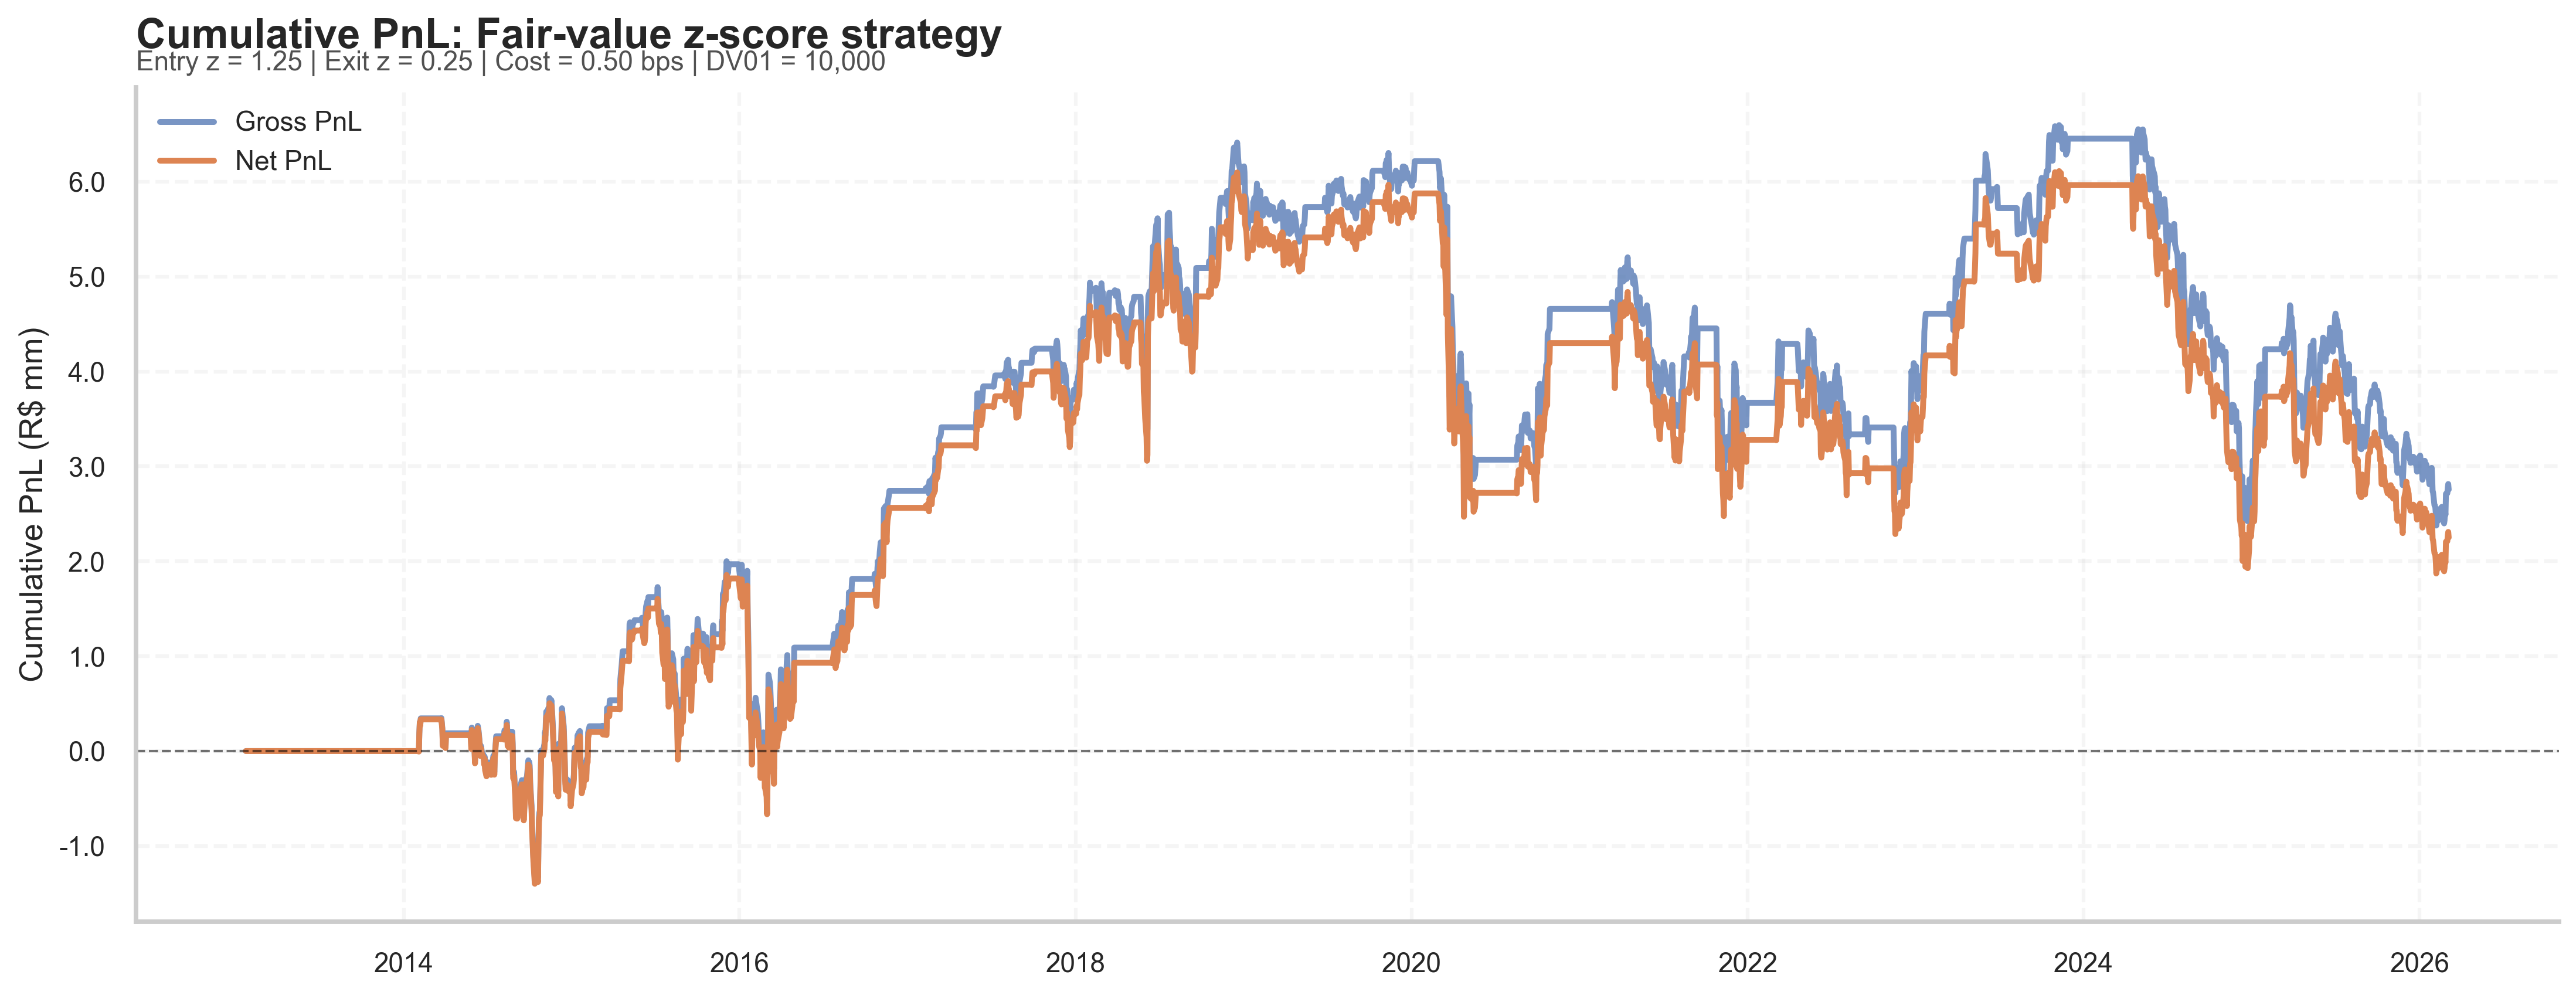
\includegraphics[width=0.92\textwidth]{figures/fig_13_cumulative_pnl_fair_value_zscore.png}
		\caption{Cumulative gross and net PnL of the fair-value z-score strategy.}
		\label{fig:cum_pnl_fv}
	\end{figure}
	
	The PnL decomposition is reported in Table \ref{tab:pnl_decomp_fv}. A relevant result is that the strategy's gains are driven primarily by realized market moves rather than by carry or rolldown. In fact, the carry/rolldown component is negative over the sample, which suggests that the framework earns money mainly when spread dislocations mean-revert rather than by passively harvesting curve carry.
	
	\begin{table}[H]
		\centering
		\footnotesize
		\resizebox{\textwidth}{!}{
			\begin{tabular}{rrrrrrr}
\toprule
Gross PnL & Carry / rolldown PnL & Market-move PnL & Transaction cost & Net PnL & Carry share of gross & Market share of gross \\
\midrule
2755927.7898 & -999689.2695 & 3755617.0593 & 505000.0000 & 2250927.7898 & -0.3627 & 1.3627 \\
\bottomrule
\end{tabular}

		}
		\caption{Stylized PnL decomposition of the fair-value z-score strategy.}
		\label{tab:pnl_decomp_fv}
	\end{table}
	
	This is an important economic result. It indicates that the strategy is best understood as a medium-frequency relative-value framework designed to exploit spread normalization episodes, not as a carry strategy.
	
	\subsection{Risk Profile}
	\label{subsec:risk_profile}
	
	Although the cumulative PnL finishes positive, the path is uneven and the drawdowns are deep. Figure \ref{fig:drawdown_fv} shows the drawdown profile of the strategy.
	
	\begin{figure}[H]
		\centering
		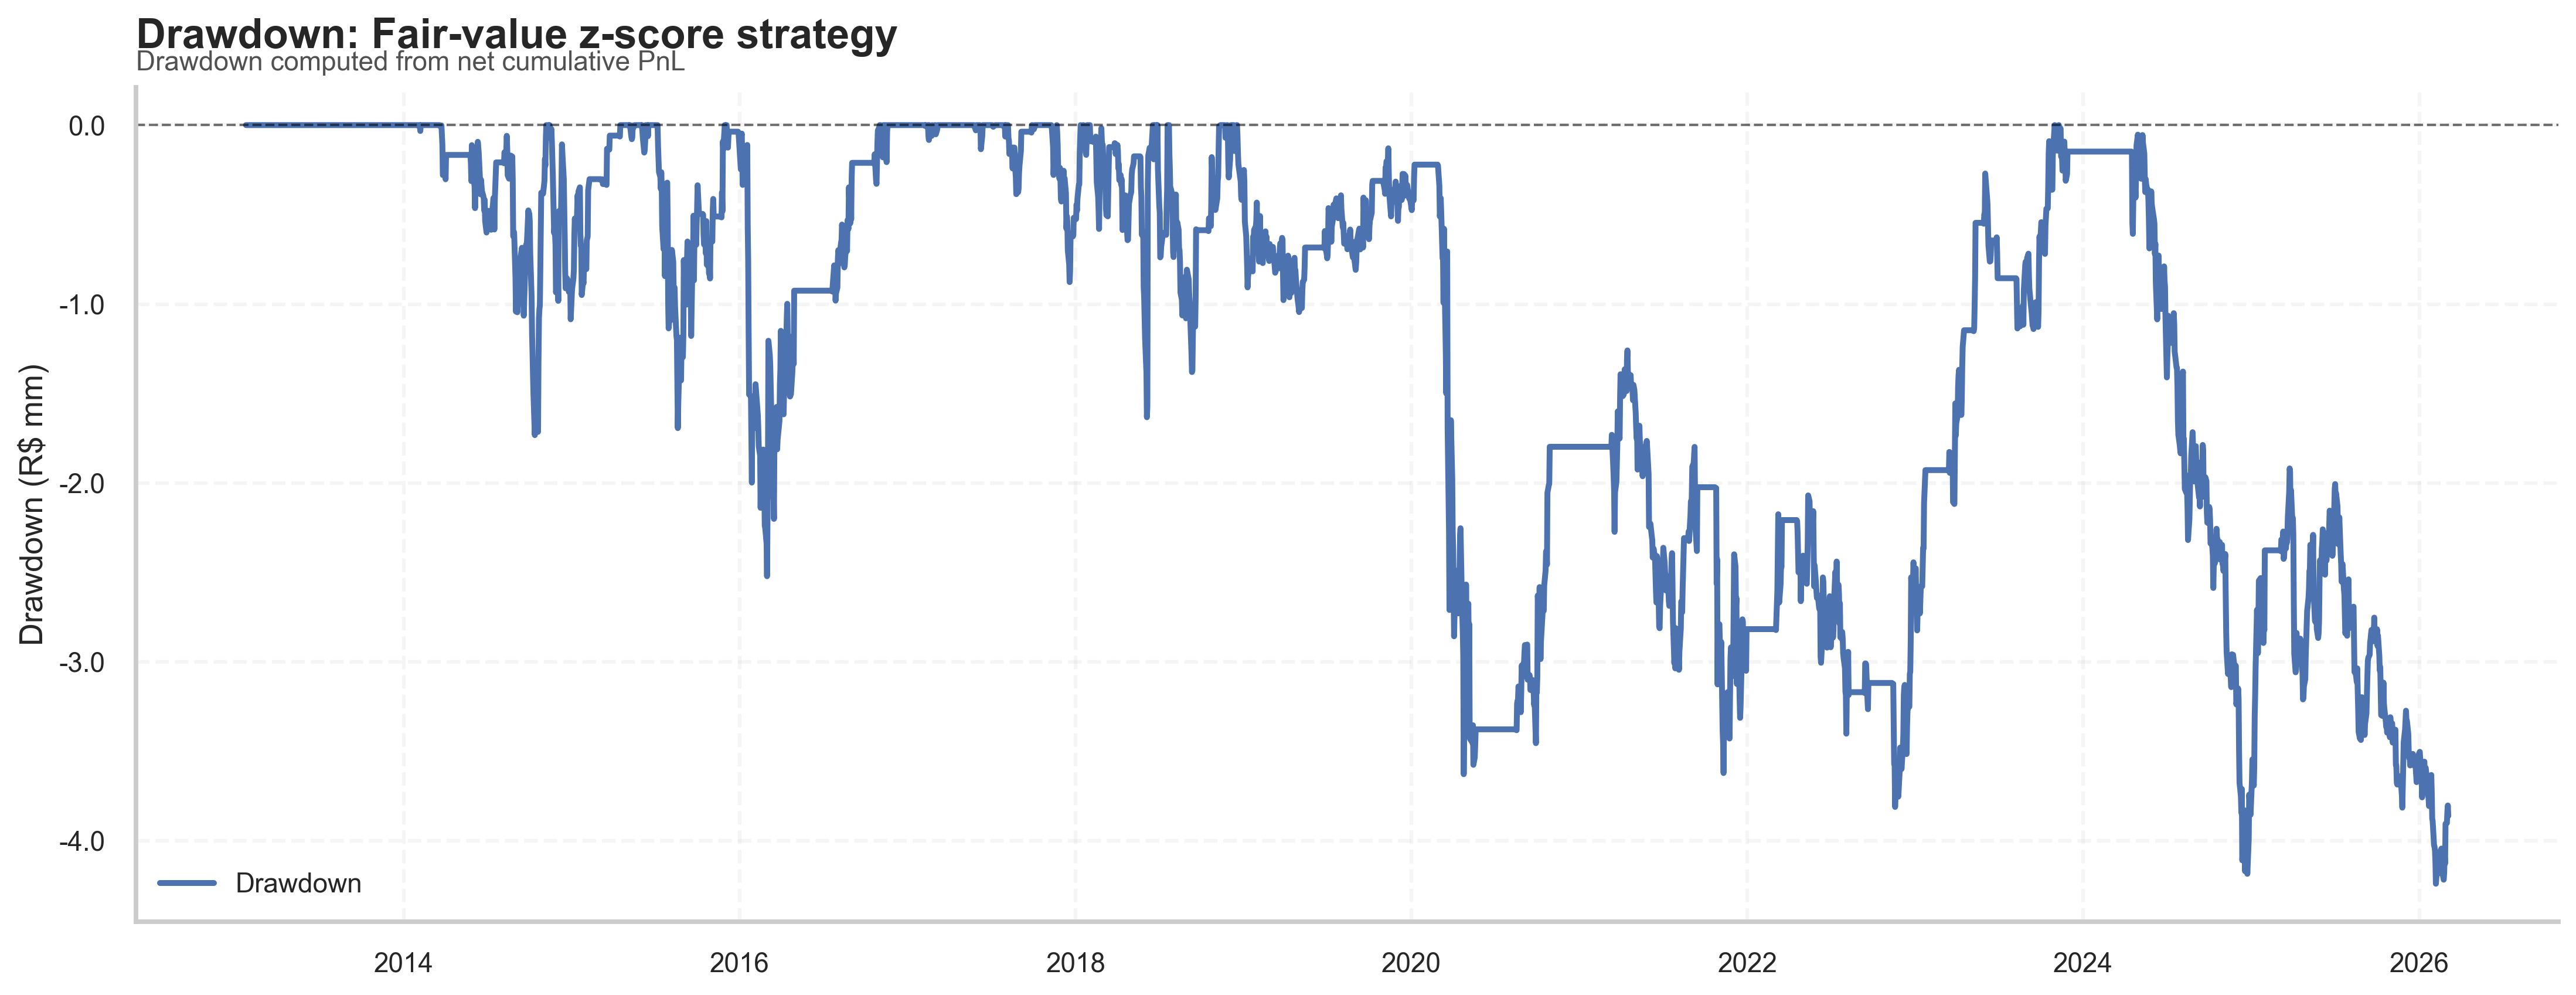
\includegraphics[width=0.92\textwidth]{figures/fig_14_drawdown_fair_value_zscore.png}
		\caption{Drawdown profile of the fair-value z-score strategy.}
		\label{fig:drawdown_fv}
	\end{figure}
	
	The drawdown pattern indicates that mispricing can remain open for long periods and that macro-implied fair value is not sufficient to force rapid convergence. This is consistent with the earlier statistical evidence: the factor is economically meaningful, but spread dynamics are heavily influenced by omitted drivers and regime-specific forces.
	
	The rolling Sharpe and yearly decomposition also indicate that performance is concentrated in a subset of the sample rather than being stable throughout. Strong years are offset by long periods of weak or negative performance. This concentration is typical of regime-dependent relative-value strategies.
	
	\begin{figure}[H]
		\centering
		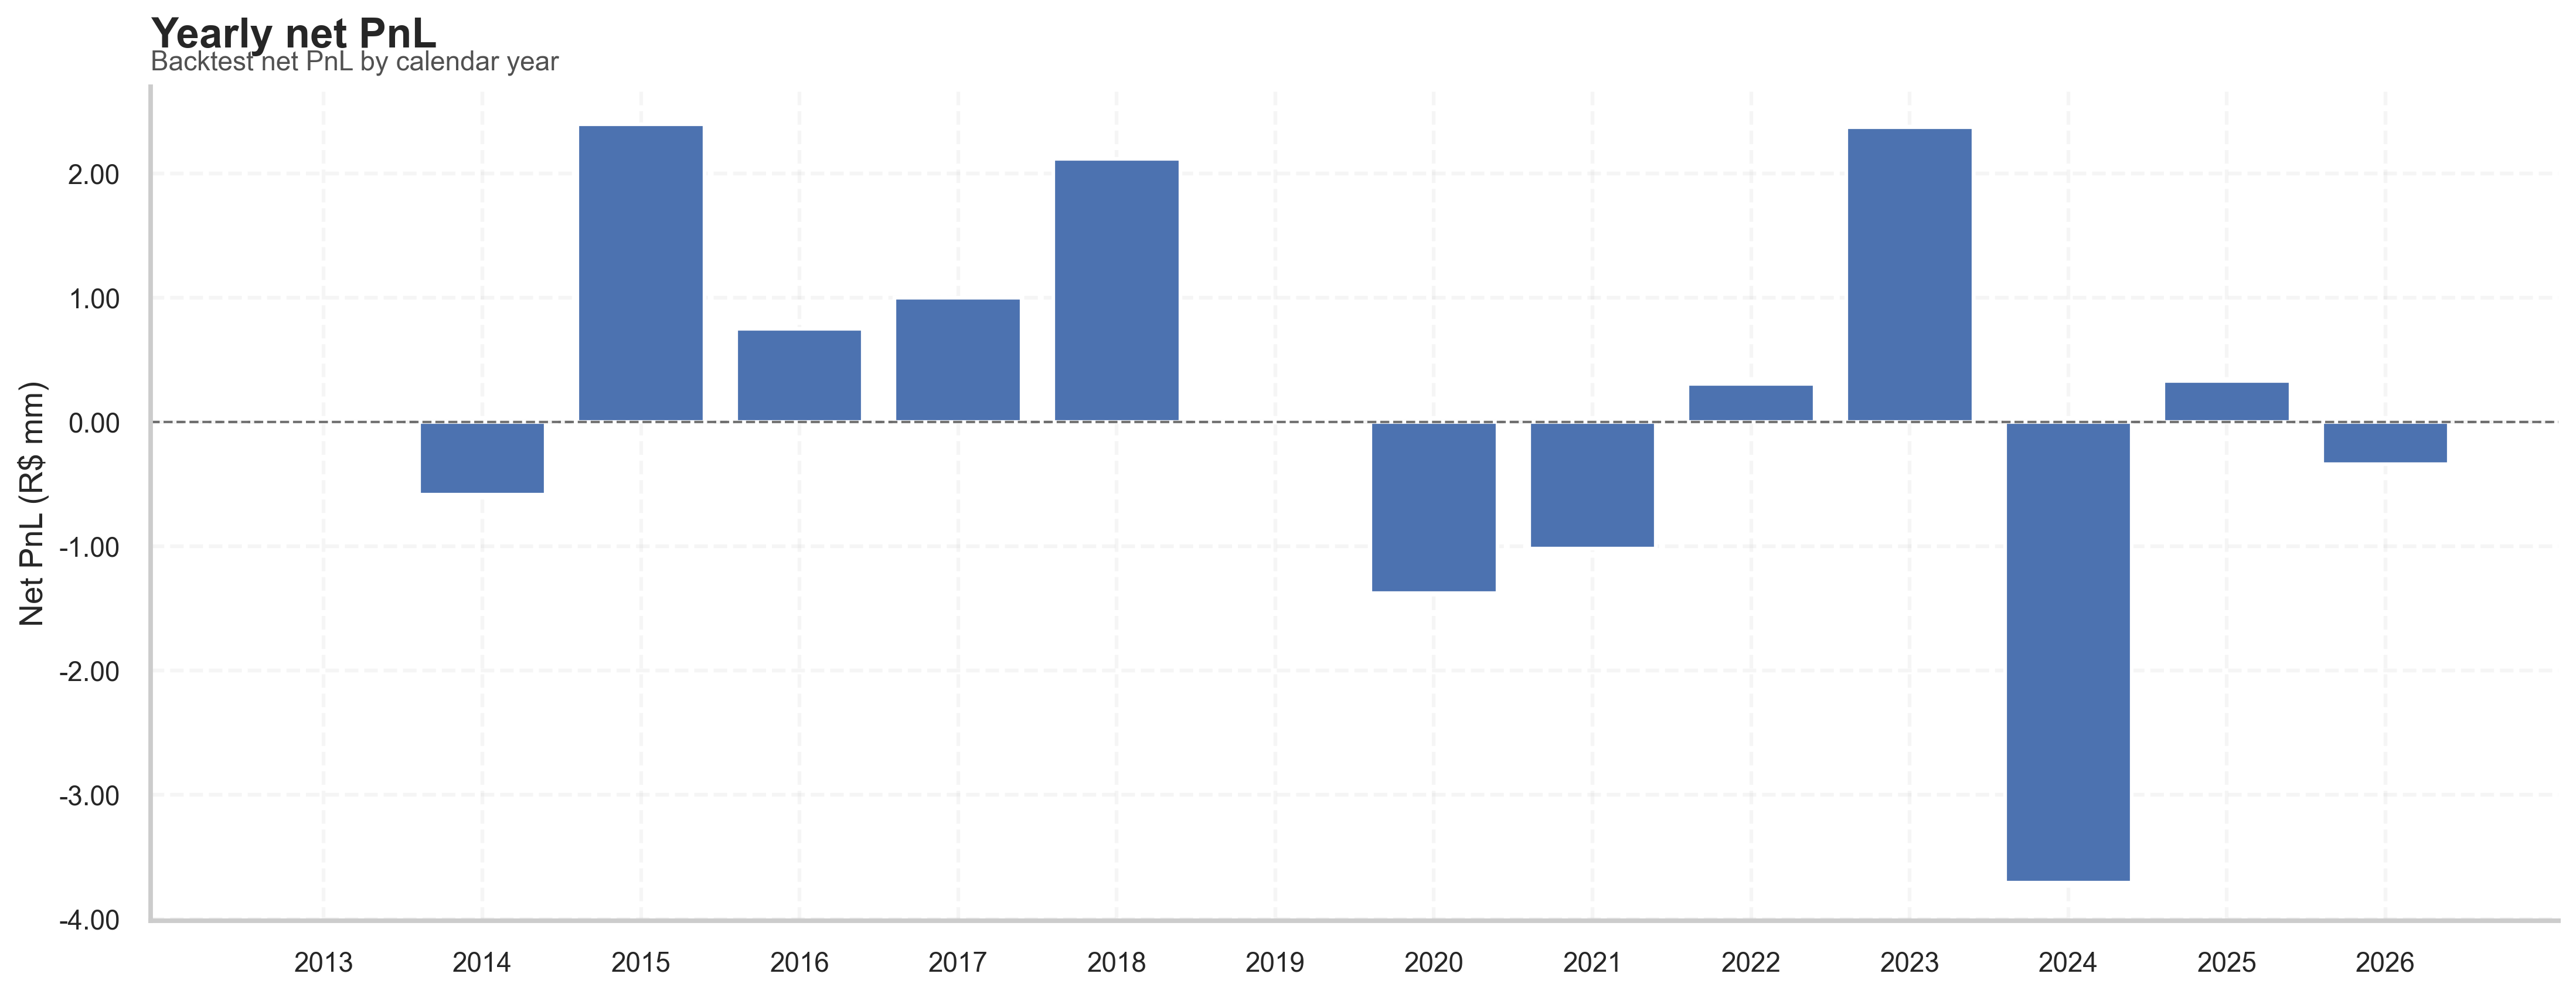
\includegraphics[width=0.88\textwidth]{figures/fig_19_yearly_pnl_fair_value_zscore.png}
		\caption{Yearly net PnL of the fair-value z-score strategy.}
		\label{fig:yearly_pnl_fv}
	\end{figure}
	
	Yearly performance confirms that the edge is not evenly distributed through time. Positive years such as 2015, 2017, 2018, and 2023 are offset by weak or negative periods such as 2020--2021 and 2024 onward. This concentration is consistent with a regime-dependent relative-value framework rather than with a stable structural alpha source.
	
	\subsection{Trade Behavior}
	\label{subsec:trade_behavior}
	
	Trade-level statistics reinforce the interpretation of the signal as a medium-frequency framework. Table \ref{tab:trade_duration_fv} reports trade-duration metrics.
	
	\begin{table}[H]
		\centering
		\footnotesize
		\resizebox{\textwidth}{!}{
			\begin{tabular}{rrrrrrrrrr}
\toprule
Number of trades & Avg holding days & Median holding days & Min holding days & Max holding days & Avg holding cal days & Median holding cal days & Profitable trades & Avg net PnL / trade & Median net PnL / trade \\
\midrule
50 & 32.80 & 19.00 & 1 & 199 & 48.34 & 29.50 & 0.64 & 74705.90 & 114257.27 \\
\bottomrule
\end{tabular}

		}
		\caption{Trade-duration statistics of the fair-value z-score strategy.}
		\label{tab:trade_duration_fv}
	\end{table}
	
	The average holding period is measured in business days and corresponds to several weeks, while the median holding period is also economically meaningful. This is fully consistent with the nature of the macro factor, which evolves more slowly than the day-to-day fluctuations of the DI curve. In other words, the strategy behaves more like a valuation-based medium-frequency relative-value process than like a short-term timing strategy.
	
	\subsection{Robustness and Threshold Sensitivity}
	\label{subsec:threshold_robustness}
	
	I also test the sensitivity of results to alternative entry and exit thresholds. The goal is not to maximize in-sample performance, but to verify whether the strategy is broadly robust to reasonable parameter changes.
	
	Table \ref{tab:threshold_sens_fv} summarizes this exercise.
	
	\begin{table}[H]
		\centering
		\footnotesize
		\resizebox{\textwidth}{!}{
			\begin{tabular}{rrrrrrrr}
\toprule
Entry z & Exit z & Obs. & Ann. PnL (R\$ k) & Ann. vol (R\$ k) & Sharpe & Max DD (R\$ k) & Turnover \\
\midrule
1.2 & 0.2 & 3252 & 174.4 & 1694.6 & 0.1 & -4240.2 & 7.8 \\
1.2 & 0.0 & 3252 & 182.8 & 1778.8 & 0.1 & -4396.7 & 6.0 \\
1.2 & 0.5 & 3252 & 9.2 & 1619.2 & 0.0 & -5757.3 & 10.0 \\
1.5 & 0.0 & 3252 & -7.0 & 1725.7 & -0.0 & -4217.8 & 4.7 \\
1.5 & 0.2 & 3252 & -14.8 & 1608.6 & -0.0 & -4156.5 & 5.7 \\
1.0 & 0.2 & 3252 & -18.6 & 1769.9 & -0.0 & -5086.4 & 10.5 \\
1.0 & 0.5 & 3252 & -39.9 & 1685.3 & -0.0 & -5830.5 & 15.3 \\
1.0 & 0.0 & 3252 & -67.7 & 1842.2 & -0.0 & -5049.5 & 7.4 \\
1.5 & 0.5 & 3252 & -80.2 & 1545.2 & -0.1 & -4810.6 & 7.4 \\
1.8 & 0.5 & 3252 & -138.8 & 1491.1 & -0.1 & -5716.7 & 5.2 \\
1.8 & 0.2 & 3252 & -145.3 & 1543.3 & -0.1 & -4947.4 & 4.0 \\
0.8 & 0.2 & 3252 & -227.6 & 1838.0 & -0.1 & -7134.7 & 15.0 \\
0.8 & 0.5 & 3252 & -242.8 & 1765.7 & -0.1 & -8012.8 & 23.0 \\
1.8 & 0.0 & 3252 & -248.6 & 1661.8 & -0.1 & -5504.7 & 3.5 \\
0.8 & 0.0 & 3252 & -284.6 & 1894.9 & -0.2 & -7041.2 & 10.0 \\
\bottomrule
\end{tabular}

		}
		\caption{Sensitivity of backtest performance to alternative z-score thresholds.}
		\label{tab:threshold_sens_fv}
	\end{table}
	
	The overall picture is one of limited robustness. The baseline configuration performs better than many neighboring alternatives, but performance is still sensitive to threshold design. This reinforces the conclusion that the signal is informative but not sufficiently strong to support aggressive standalone deployment without additional filters or broader context.
	
	\subsection{Performance Across Macro Periods}
	\label{subsec:macro_periods}
	
	The strategy's behavior varies materially across macro regimes. Performance is better in periods when the relationship between inflation, monetary-policy expectations, and curve shape is more orderly. By contrast, performance deteriorates sharply in periods dominated by non-linear shocks, abrupt policy repricing, fiscal risk, or long-end term-premium movements.
	
	\begin{figure}[H]
		\centering
		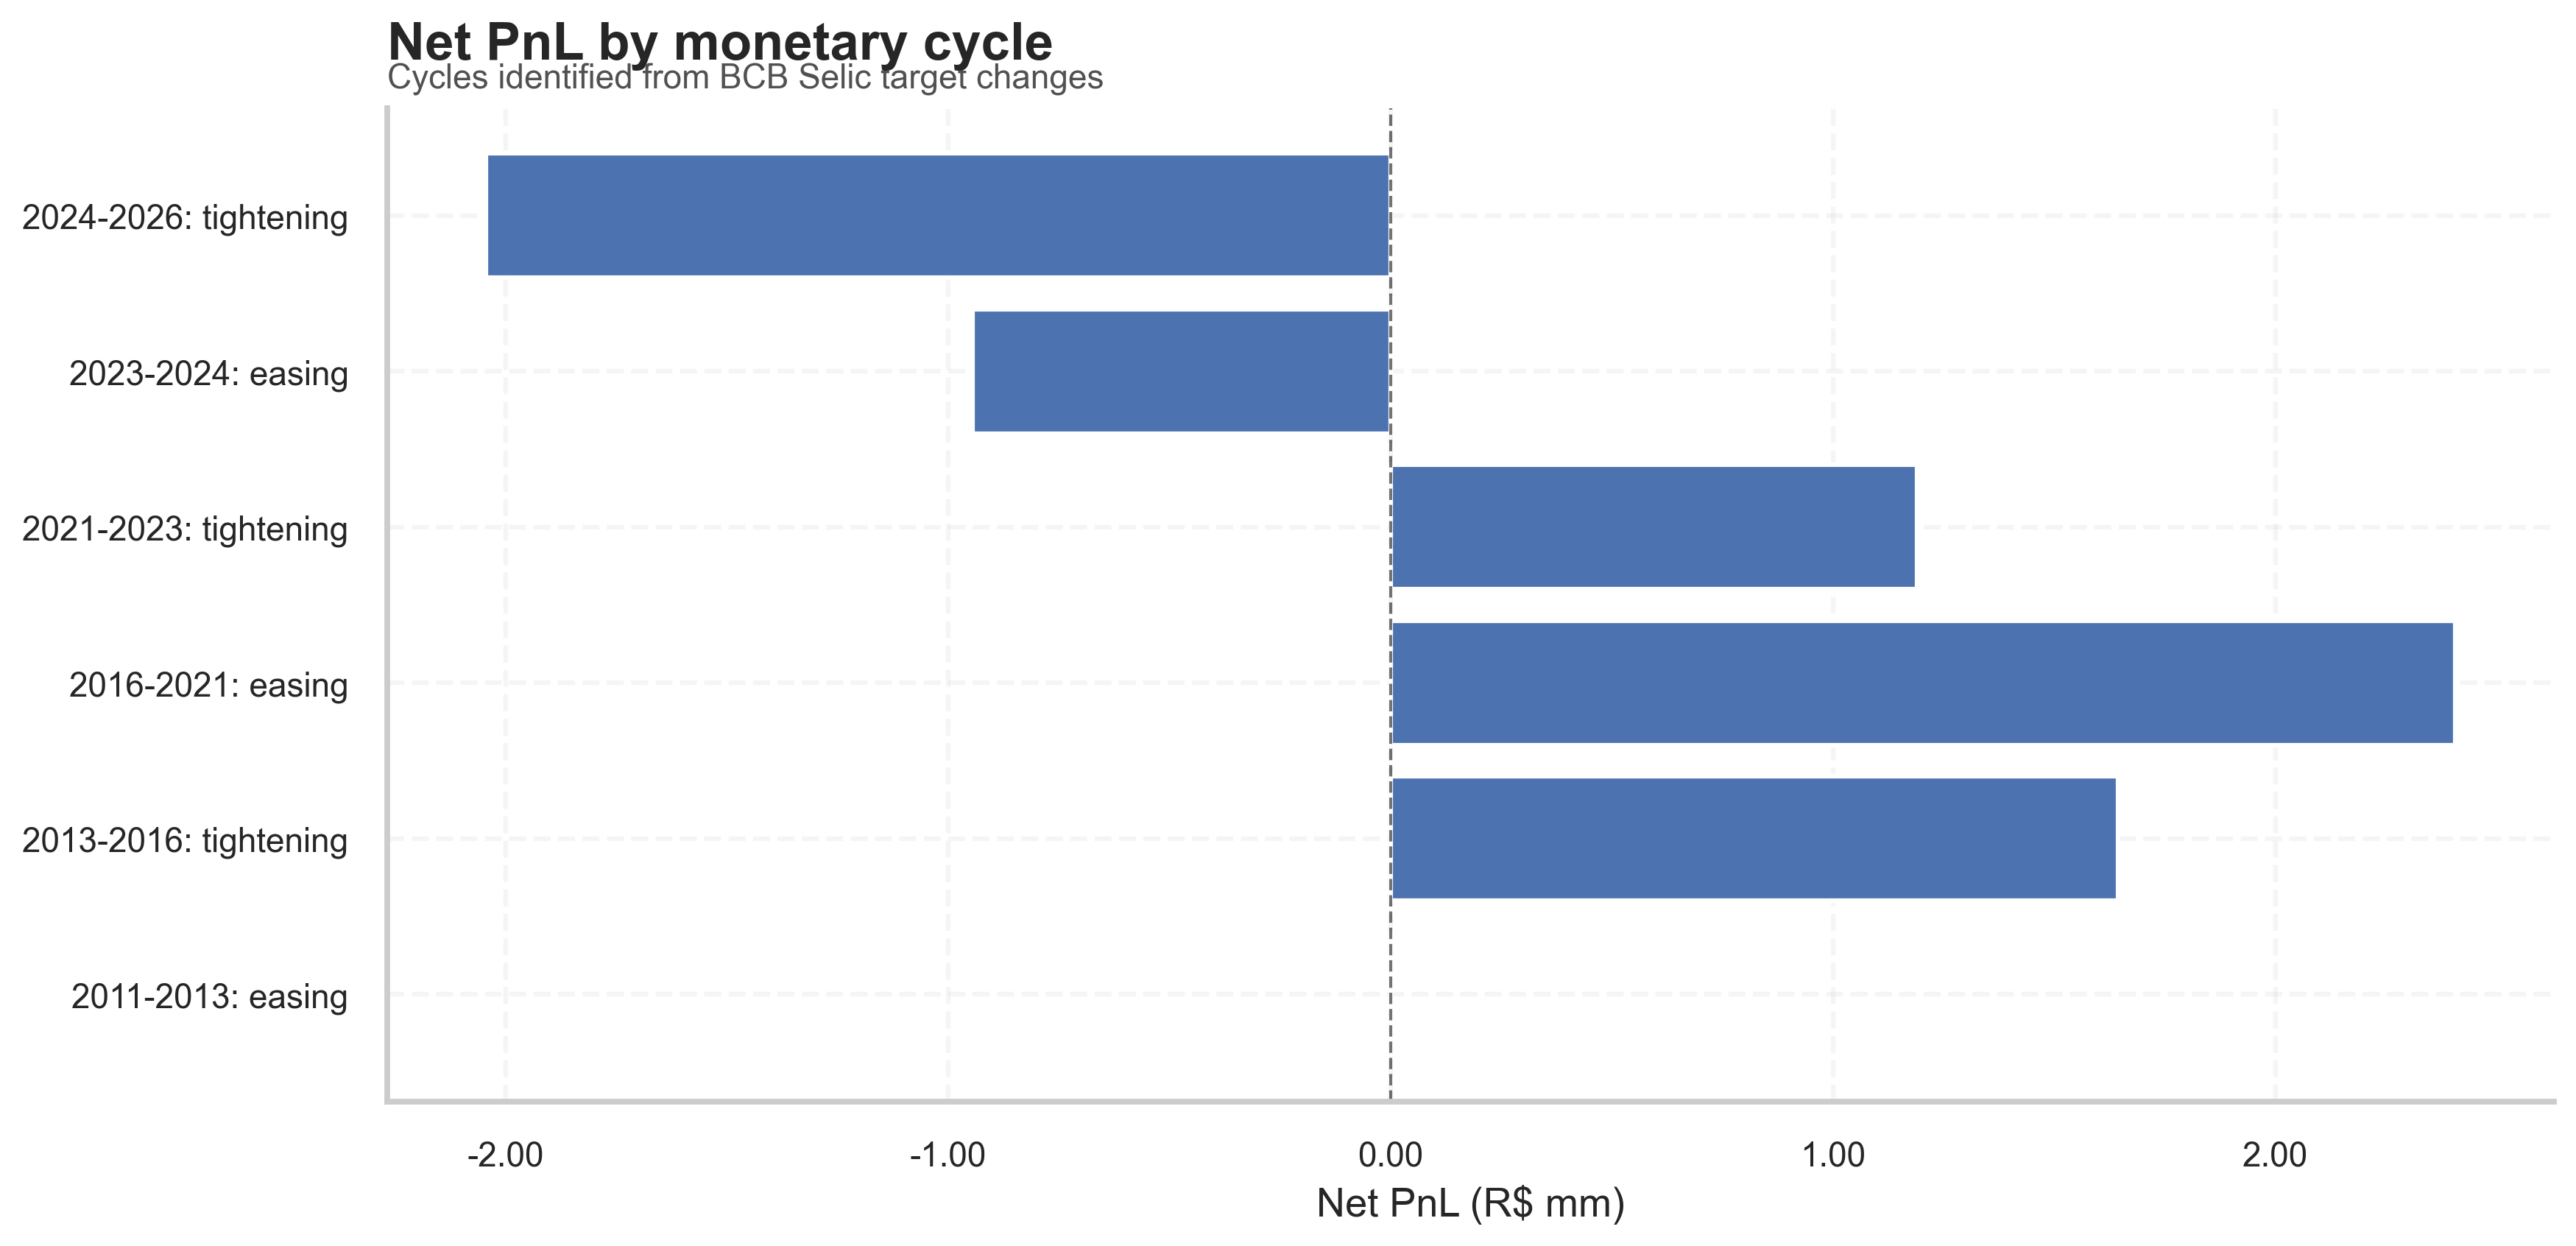
\includegraphics[width=0.92\textwidth]{figures/fig_21_pnl_by_monetary_cycle.png}
		\caption{Net PnL of the fair-value z-score strategy grouped by monetary-policy cycles identified from changes in the BCB Selic target.}
		\label{fig:pnl_monetary_cycle}
	\end{figure}
	
	\begin{table}[H]
		\centering
		\footnotesize
		\resizebox{\textwidth}{!}{
			\begin{tabular}{llllrrrrrrrrrrr}
\toprule
Monetary cycle & Start & End & Type & Obs. & Total PnL & Mean daily PnL & Daily vol & Annualized PnL & Annualized vol & Sharpe & Max drawdown & Avg |position| & Annual turnover & Hit ratio \\
\midrule
2011-2013: easing & 2011-09-01 & 2013-04-17 & easing & 57 & 0.0000 & 0.0000 & 0.0000 & 0.0000 & 0.0000 &  & 0.0000 & 0.0000 & 0.0000 & 0.0000 \\
2013-2016: tightening & 2013-04-18 & 2016-10-19 & tightening & 870 & 1644973.4310 & 1890.7741 & 104549.9043 & 476475.0628 & 1659678.2784 & 0.2871 & -2521352.5568 & 0.4575 & 9.8483 & 0.2322 \\
2016-2021: easing & 2016-10-20 & 2021-03-17 & easing & 1086 & 2407371.1881 & 2216.7322 & 111414.1842 & 558616.5188 & 1768645.3438 & 0.3158 & -3627950.7424 & 0.5773 & 9.0497 & 0.2974 \\
2021-2023: tightening & 2021-03-18 & 2023-08-02 & tightening & 594 & 1189634.3024 & 2002.7514 & 111935.4753 & 504693.3404 & 1776920.5828 & 0.2840 & -3810888.4515 & 0.5741 & 9.7576 & 0.2912 \\
2023-2024: easing & 2023-08-03 & 2024-09-18 & easing & 283 & -944867.6173 & -3338.7548 & 89117.8496 & -841366.2176 & 1414702.0052 & -0.5947 & -2319214.4262 & 0.6537 & 2.6714 & 0.2862 \\
2024-2026: tightening & 2024-09-19 & 2026-03-05 & tightening & 362 & -2046183.5143 & -5652.4406 & 110237.2588 & -1424415.0431 & 1749962.2324 & -0.8140 & -4240165.1137 & 0.9365 & 1.3923 & 0.4779 \\
\bottomrule
\end{tabular}

		}
		\caption{Performance of the fair-value z-score framework across monetary-policy cycles identified from the BCB Selic target series.}
		\label{tab:monetary_cycle_metrics}
	\end{table}
	
	Grouping performance by monetary-policy cycle helps clarify the economic nature of the strategy. Cycles are identified mechanically from changes in the BCB Selic target series, so the classification does not rely on ex-post qualitative judgment. The results suggest that the fair-value z-score framework performs better in more orderly monetary-policy environments, when the connection between inflation expectations, policy repricing, and the shape of the forward DI curve remains relatively coherent. In those periods, deviations between the observed spread and its macro-implied fair value are more likely to mean-revert. By contrast, performance deteriorates in episodes of abrupt regime shifts or strong non-macro shocks, when the spread can remain persistently away from the model-implied anchor.
	
	\begin{figure}[H]
		\centering
		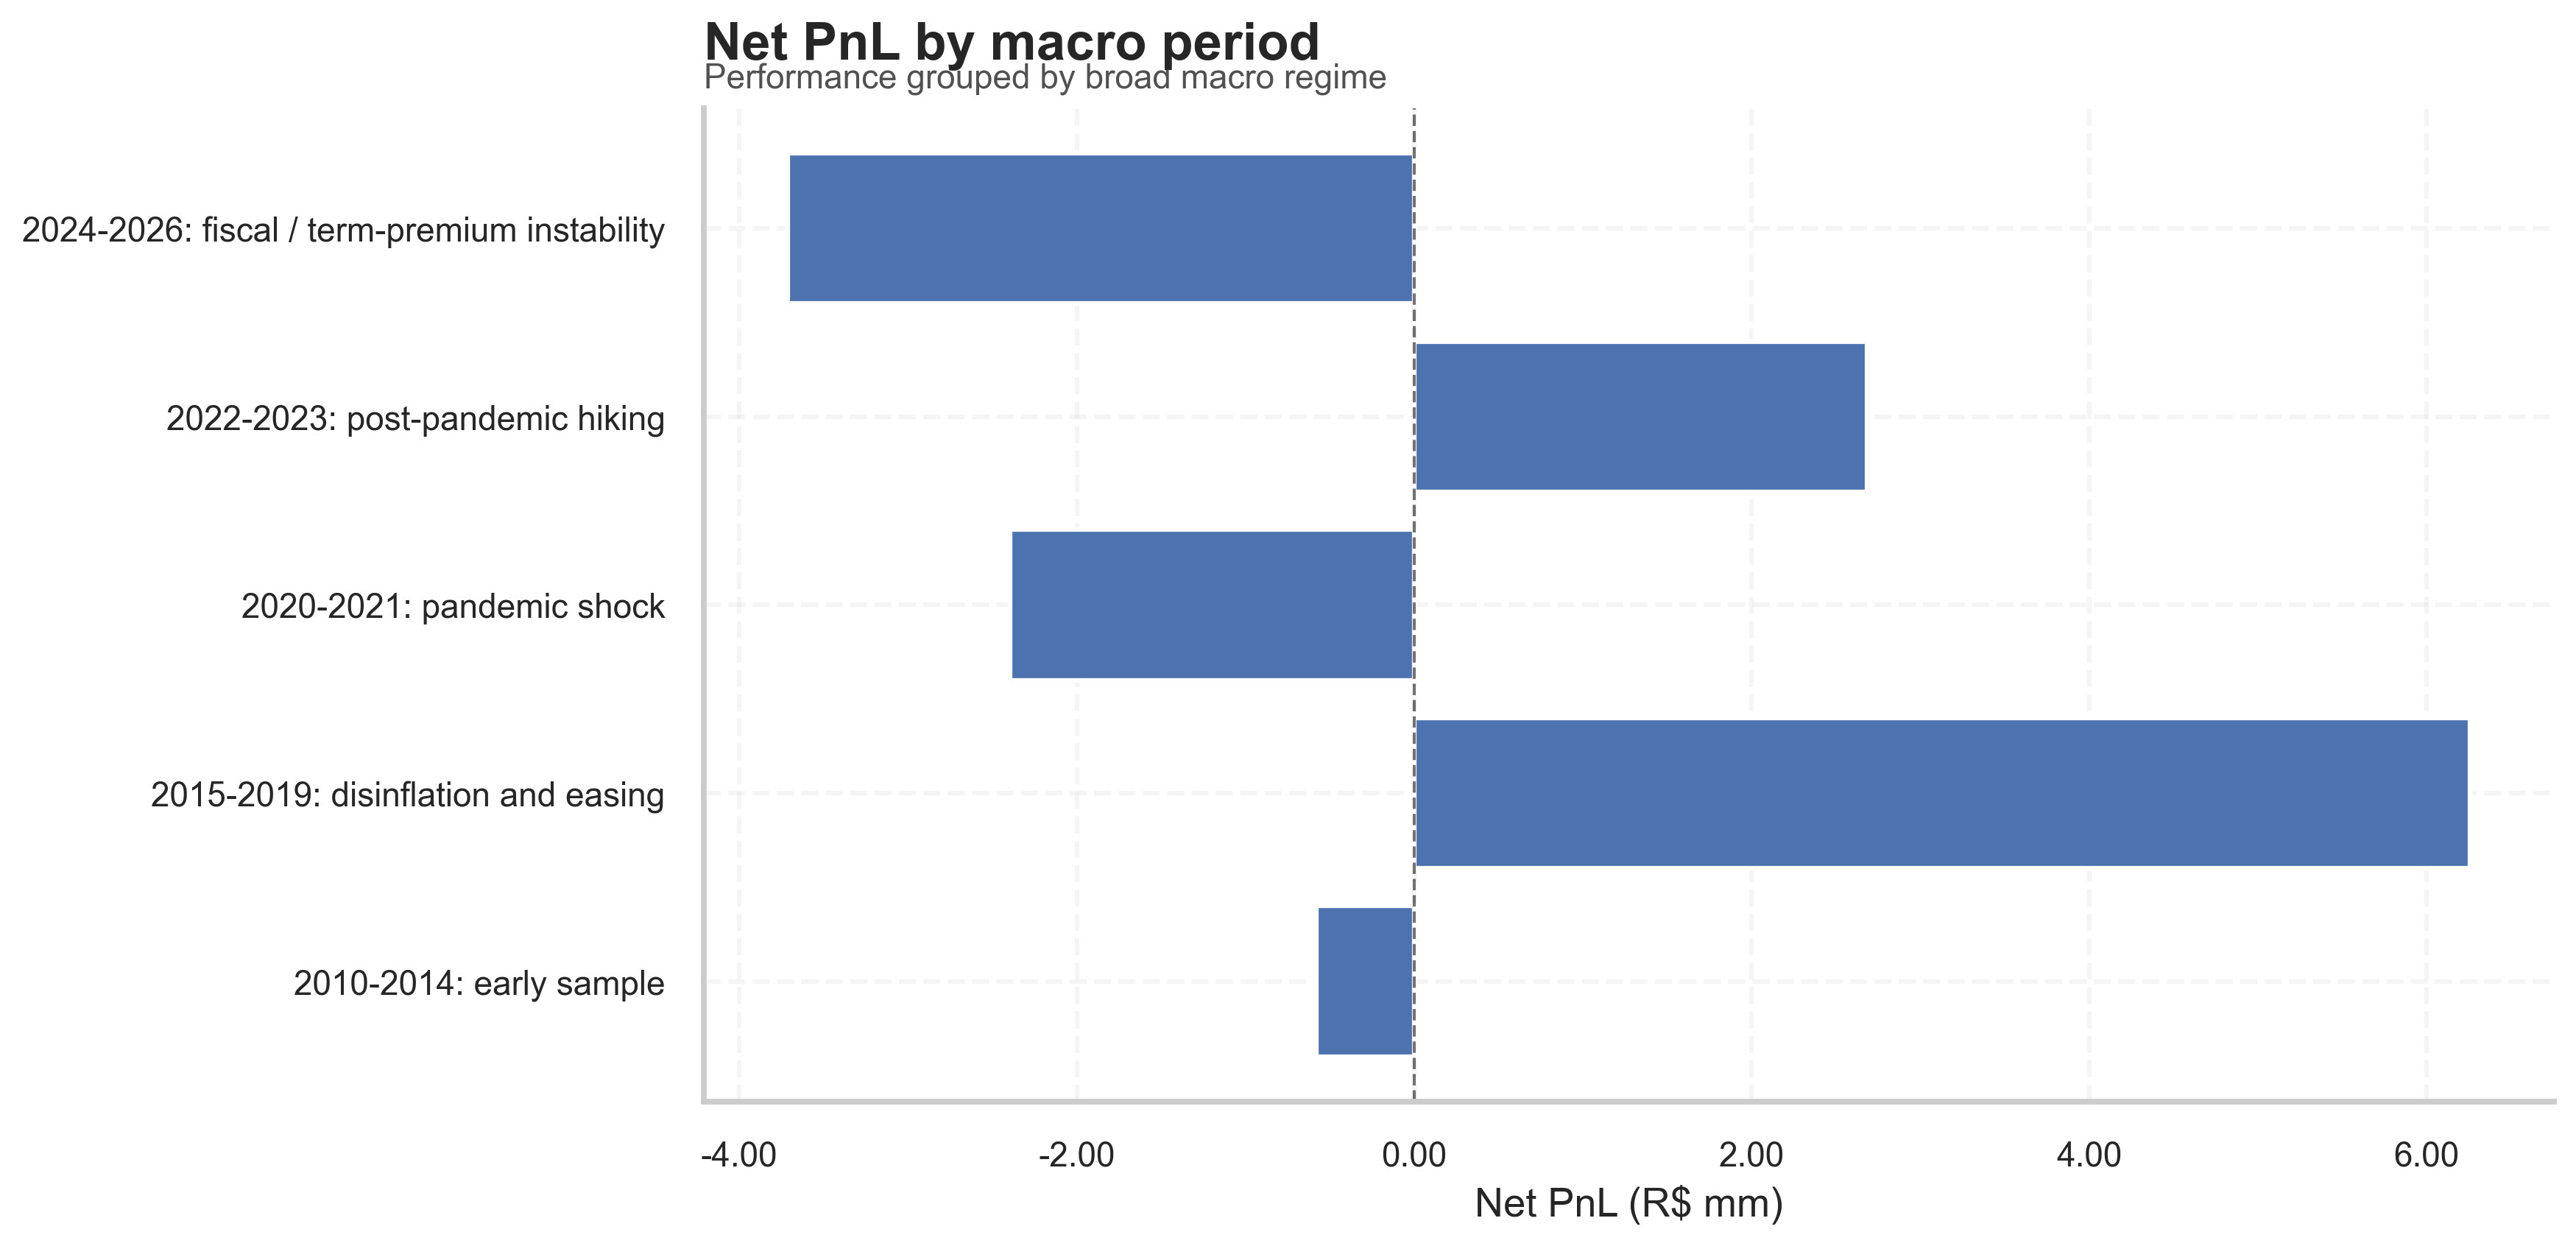
\includegraphics[width=0.92\textwidth]{figures/fig_20_period_pnl_fair_value_zscore.png}
		\caption{Net PnL of the fair-value z-score strategy grouped by broad macro periods.}
		\label{fig:pnl_macro_period}
	\end{figure}
	
	The same conclusion appears when performance is grouped by broader macro periods rather than by policy-cycle turning points alone. The framework tends to behave better in post-recession disinflation and easing environments, when deviations between the observed spread and macro-implied fair value are more likely to converge. It behaves worse in periods such as the pandemic and reopening phase, when the DI curve is influenced not only by inflation and activity, but also by abrupt policy changes, liquidity effects, fiscal-risk premia, and long-end term-premium shocks.
	
	Figures \ref{fig:pnl_monetary_cycle} and \ref{fig:pnl_macro_period} therefore provide two complementary views of the same result: performance is highly regime-dependent, and the signal appears to work better when the connection between macro fundamentals and forward-curve valuation is more orderly.
	
	Taken together, the monetary-cycle and macro-period decompositions point to the same conclusion. The signal is economically meaningful, but its performance depends critically on whether the DI curve is being priced primarily through inflation and monetary-policy expectations or through other omitted drivers such as fiscal credibility, long-end term-premium shocks, global rates, and liquidity conditions. The strategy therefore works better as a conditional macro valuation framework than as an unconditional spread-trading rule.
	
	\subsection{Rolling Cointegration as a Regime Diagnostic}
	\label{subsec:rolling_cointegration}
	
	As an additional structural diagnostic, I evaluate rolling Engle--Granger cointegration between the two forward legs \(5y5y\) and \(1y1y\). The idea is straightforward: if the two forwards are tightly linked by a stable long-run relationship, then spread deviations may be better interpreted as equilibrium dislocations; if that relationship weakens, the spread is more likely to reflect broader macro, fiscal, or term-premium shocks.
	
	Figure \ref{fig:rolling_coint_pvalue} reports the rolling cointegration p-value. Strong cointegration is episodic rather than persistent. Using a 252-business-day rolling window and a 5-day step, windows classified as strong, moderate, and weak cointegration account for roughly 3.3\%, 9.7\%, and 9.8\% of the sample, respectively, while 77.2\% of the sample falls into the non-cointegrated regime.
	
	\begin{figure}[H]
		\centering
		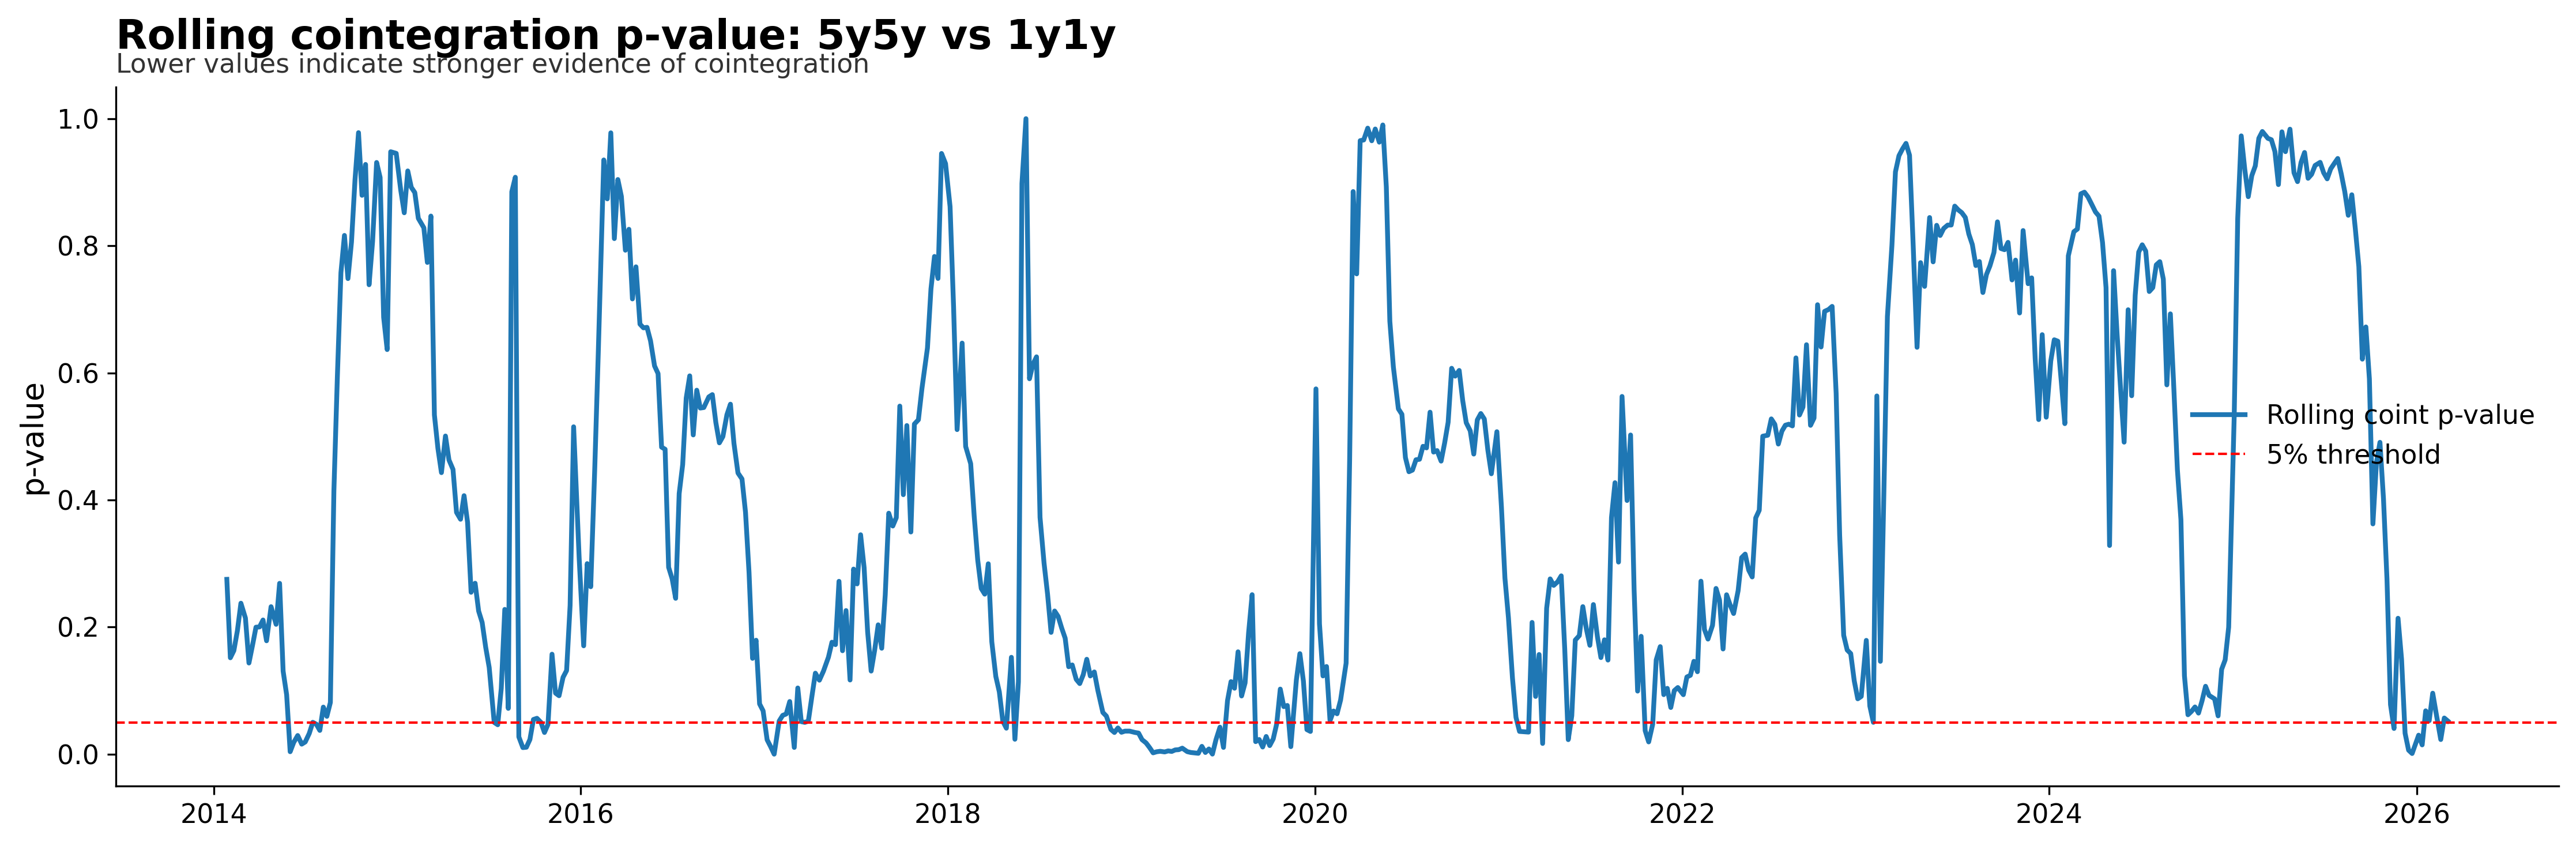
\includegraphics[width=0.92\textwidth]{figures/05_cointegration/fig_23_rolling_cointegration_pvalue.png}
		\caption{Rolling Engle--Granger p-value for cointegration between \(5y5y\) and \(1y1y\). Lower values indicate stronger evidence of cointegration.}
		\label{fig:rolling_coint_pvalue}
	\end{figure}
	
	This helps explain why a pure cointegration-only trading rule proved too restrictive in implementation: the strongest equilibrium-type windows are relatively rare and therefore generate low trade frequency and low capital utilization.
	
	More importantly, performance grouped by cointegration regime indicates that positive net PnL is concentrated in non-cointegrated windows rather than in the strongly cointegrated states.
	
	\begin{figure}[H]
		\centering
		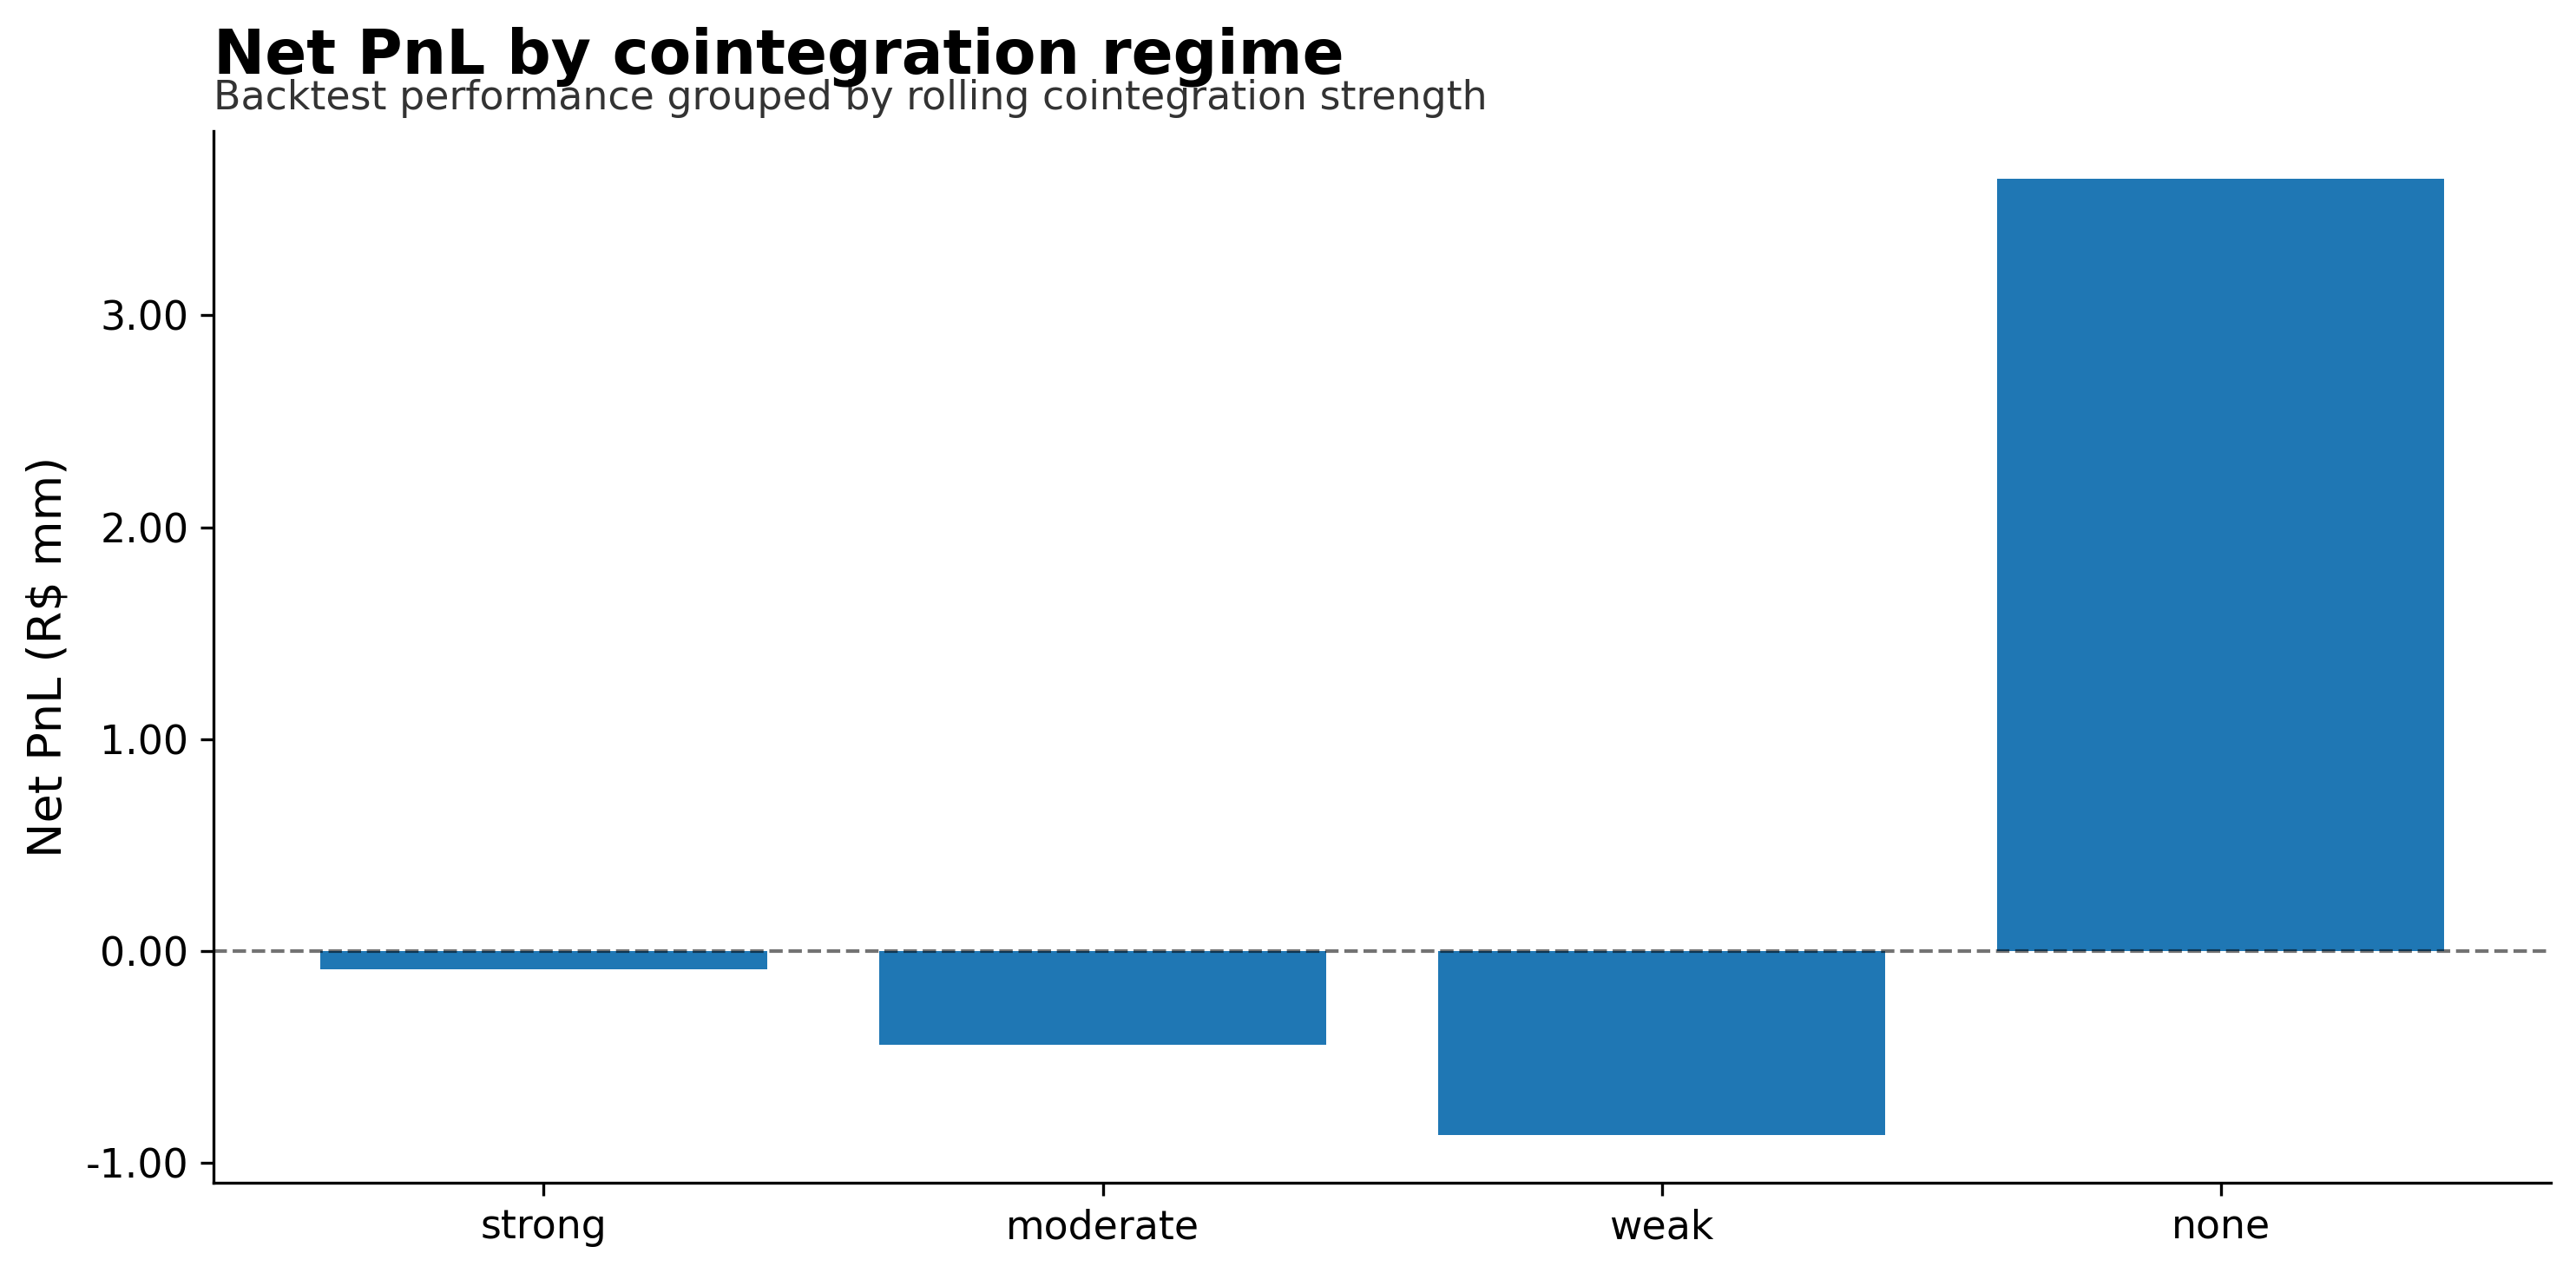
\includegraphics[width=0.92\textwidth]{figures/05_cointegration/fig_26_pnl_by_cointegration_regime.png}
		\caption{Net PnL grouped by rolling cointegration regime.}
		\label{fig:pnl_cointegration_regime}
	\end{figure}
	
	The result is economically informative. The strong, moderate, and weak cointegration regimes contribute approximately \(-\)R\$0.09 million, \(-\)R\$0.44 million, and \(-\)R\$0.87 million of net PnL, respectively, whereas the non-cointegrated regime contributes approximately \(+\)R\$3.65 million. This suggests that the main monetizable opportunities in the spread do not arise when the two forward legs are tightly anchored by a stable long-run equilibrium. Instead, the fair-value framework monetizes better when that linkage weakens and the spread becomes more exposed to broader macro repricing, fiscal risk, global rates, and term-premium variation.
	
	Rolling cointegration is therefore useful as a structural regime diagnostic and as supporting evidence on market structure, but not as the primary trading engine. In the final framework, I retain the fair-value z-score implementation as the main specification and interpret cointegration mainly as a complementary filter or robustness lens.
	
	\section{Economic Interpretation, Limitations, and Conclusion}
	\label{sec:limitations_conclusion}
	
	\subsection{Economic Interpretation}
	\label{subsec:economic_interpretation}
	
	The main contribution of this case is not the discovery of a high-Sharpe standalone trading rule. Rather, it is the construction of a coherent macro-to-rates framework for the Brazilian DI curve.
	
	The evidence suggests that the inflation expectations gap is economically relevant for the forward slope spread, but mainly through a \emph{valuation channel}. In other words, the macro factor helps anchor where the spread should trade on a medium-frequency basis, even if it does not forecast short-horizon daily changes with high precision.
	
	This is consistent with how macro information often enters rates trading in practice. Inflation-related variables do not necessarily predict tomorrow's mark-to-market, but they do provide a useful reference point for identifying when parts of the curve look rich or cheap relative to the macro backdrop.
	
	The cointegration exercise refines that interpretation. When the structural linkage between \(5y5y\) and \(1y1y\) is very tight, monetizable dislocations appear to be rarer. When that linkage weakens, the spread becomes more exposed to medium-frequency macro and term-premium shocks, and the fair-value framework becomes more relevant as a valuation anchor.
	
	\subsection{Why the Strategy Struggles in Some Periods}
	\label{subsec:why_strategy_struggles}
	
	The weakest phase of the framework coincides with periods in which the DI curve was dominated by drivers not fully captured by the simple inflation-based model.
	
	The pandemic and reopening period is the clearest example. During 2020--2021, the curve was influenced by a combination of:
	\begin{itemize}
		\item abrupt collapse and rebound in growth expectations,
		\item emergency monetary easing followed by aggressive repricing,
		\item inflation shocks with highly non-linear pass-through,
		\item fiscal uncertainty and changing sovereign-risk perceptions,
		\item term-premium and liquidity effects, especially at longer horizons.
	\end{itemize}
	
	Under those conditions, the spread could remain persistently away from macro-implied fair value for longer than the strategy could tolerate. A similar issue can arise in more recent periods when the long end is heavily influenced by fiscal credibility and global rates rather than by the simple inflation-versus-realization framework.
	
	This helps explain why the signal is economically sensible yet still vulnerable to long drawdowns and unstable subperiod performance.
	
	\subsection{Main Limitations}
	\label{subsec:main_limitations}
	
	The framework has several important limitations.
	
	First, the fair value is model-implied rather than structural. It should be interpreted as a useful macro anchor, not as a true equilibrium spread.
	
	Second, the backtest is stylized. PnL is computed at the spread level using a fixed spread-DV01 convention rather than a full instrument-level implementation with exact hedge ratios, contract selection, financing, and execution constraints.
	
	Third, the carry/rolldown decomposition is approximate. It is intended to separate passive carry from realized spread repricing, but it is not a full production-quality decomposition.
	
	Fourth, the signal is regime-dependent. Rolling regressions, yearly performance, macro-period analysis, and the cointegration diagnostics all indicate that the relationship between macro and spread dynamics is not stable across time.
	
	Finally, the model omits important drivers of the Brazilian curve, including fiscal credibility, external rates, risk premium variation, and market-technical effects.
	
	\subsection{Final Conclusion}
	\label{subsec:final_conclusion}
	
	This case studies whether inflation-related macro information helps explain and trade the forward slope of the Brazilian DI curve, measured as
	\[
	5y5y - 1y1y.
	\]
	
	The empirical results lead to a nuanced conclusion.
	
	The macro hypothesis is economically coherent, the data construction is internally consistent, and the no-look-ahead alignment is carefully handled. However, the inflation expectations gap is weak as a standalone predictor of short-horizon spread changes. The more useful interpretation is a fair-value one: macro data help define a medium-frequency valuation anchor for the spread, and trading opportunities arise when the observed spread deviates materially from that anchor.
	
	The resulting fair-value z-score strategy produces some positive cumulative performance, but with low Sharpe, substantial drawdowns, and meaningful parameter sensitivity. Rolling cointegration between \(5y5y\) and \(1y1y\) adds useful structural information, but its strongest regimes are too episodic and too restrictive to serve as the main implementation rule. As a result, the framework is better viewed as a macro valuation and regime-conditioning tool than as a robust standalone alpha strategy.
	
	In practical terms, the most promising next step would be to enrich the framework with additional drivers --- especially fiscal, external-rates, and term-premium variables --- and to embed the fair-value signal into a broader relative-value process rather than using it in isolation.
	
	\appendix
	
	\section{Additional Tables and Diagnostics}
	
	\begin{table}[H]
		\centering
		\footnotesize
		\resizebox{\textwidth}{!}{
			\begin{tabular}{rrrrrrrrrrrr}
\toprule
Year & Obs. & Total PnL & Mean daily PnL & Daily vol & Annualized PnL & Annualized vol & Sharpe & Max drawdown & Avg |position| & Annual turnover & Hit ratio \\
\midrule
2013 & 233 & 0.00 & 0.00 & 0.00 & 0.00 & 0.00 &  & 0.00 & 0.00 & 0.00 & 0.00 \\
2014 & 248 & -581558.07 & -2344.99 & 103902.68 & -590938.04 & 1649403.84 & -0.36 & -1732614.55 & 0.58 & 11.18 & 0.27 \\
2015 & 246 & 2395633.20 & 9738.35 & 115056.06 & 2454063.28 & 1826458.36 & 1.34 & -1693587.49 & 0.58 & 20.49 & 0.32 \\
2016 & 249 & 749220.69 & 3008.92 & 125229.02 & 758247.45 & 1987949.11 & 0.38 & -2521352.56 & 0.53 & 5.06 & 0.28 \\
2017 & 246 & 999703.78 & 4063.84 & 50036.18 & 1024086.80 & 794299.79 & 1.29 & -877345.97 & 0.40 & 13.32 & 0.23 \\
2018 & 244 & 2116989.97 & 8676.19 & 135794.83 & 2186399.48 & 2155676.16 & 1.01 & -1632885.30 & 0.79 & 14.46 & 0.39 \\
2019 & 248 & -4787.44 & -19.30 & 68744.45 & -4864.66 & 1091284.31 & -0.00 & -1044918.35 & 0.81 & 4.06 & 0.40 \\
2020 & 249 & -1375376.38 & -5523.60 & 165748.00 & -1391947.18 & 2631167.98 & -0.53 & -3627950.74 & 0.44 & 5.06 & 0.22 \\
2021 & 247 & -1019170.03 & -4126.19 & 126637.75 & -1039801.01 & 2010311.92 & -0.52 & -3621468.98 & 0.67 & 6.12 & 0.31 \\
2022 & 250 & 310195.81 & 1240.78 & 101510.29 & 312677.37 & 1611425.93 & 0.19 & -3810888.45 & 0.50 & 9.07 & 0.25 \\
2023 & 248 & 2373226.73 & 9569.46 & 79681.58 & 2411504.58 & 1264905.86 & 1.91 & -2824432.67 & 0.52 & 11.18 & 0.29 \\
2024 & 251 & -3706602.85 & -14767.34 & 106058.75 & -3721370.20 & 1683630.50 & -2.21 & -4184865.14 & 0.71 & 1.00 & 0.29 \\
2025 & 250 & 331858.18 & 1327.43 & 107105.42 & 334513.04 & 1700245.90 & 0.20 & -3815005.62 & 0.91 & 2.02 & 0.50 \\
2026 & 43 & -338405.79 & -7869.90 & 82451.80 & -1983215.30 & 1308881.82 & -1.52 & -4240165.11 & 1.00 & 0.00 & 0.47 \\
\bottomrule
\end{tabular}

		}
		\caption{Yearly performance metrics of the fair-value z-score strategy.}
		\label{tab:yearly_metrics_appendix}
	\end{table}
	
	\begin{table}[H]
		\centering
		\footnotesize
		\resizebox{\textwidth}{!}{
			\begin{tabular}{lllrrrrrrrrrrr}
\toprule
Period & Start & End & Obs. & Total PnL & Mean daily PnL & Daily vol & Annualized PnL & Annualized vol & Sharpe & Max drawdown & Avg |position| & Annual turnover & Hit ratio \\
\midrule
2010-2014: early sample & 2013-01-22 & 2014-12-30 & 481 & -581558.0706 & -1209.0604 & 74543.2592 & -304683.2303 & 1183337.5542 & -0.2575 & -1732614.5549 & 0.3008 & 5.7510 & 0.1414 \\
2015-2019: disinflation and easing & 2015-01-02 & 2019-12-30 & 1233 & 6256760.2013 & 5074.4203 & 104331.5093 & 1278753.9098 & 1656211.3654 & 0.7721 & -2521352.5568 & 0.6212 & 11.4453 & 0.3244 \\
2020-2021: pandemic shock & 2020-01-02 & 2021-12-30 & 496 & -2394546.4170 & -4827.7146 & 147425.9190 & -1216584.0667 & 2340313.9111 & -0.5198 & -3627950.7424 & 0.5544 & 5.5887 & 0.2681 \\
2022-2023: post-pandemic hiking & 2022-01-03 & 2023-12-28 & 498 & 2683422.5373 & 5388.3987 & 91298.0130 & 1357876.4647 & 1449311.0259 & 0.9369 & -3810888.4515 & 0.5120 & 10.1205 & 0.2691 \\
2024-2026: fiscal / term-premium instability & 2024-01-02 & 2026-03-05 & 544 & -3713150.4612 & -6825.6442 & 104999.8731 & -1720062.3460 & 1666821.3122 & -1.0319 & -4240165.1137 & 0.8254 & 1.3897 & 0.3989 \\
\bottomrule
\end{tabular}

		}
		\caption{Performance metrics across broad macro periods.}
		\label{tab:macro_period_metrics_appendix}
	\end{table}
	
	\begin{table}[H]
		\centering
		\footnotesize
		\resizebox{\textwidth}{!}{
			\begin{tabular}{lrrrrrrrr}
\toprule
Period & Gross PnL & Carry / rolldown & Market move & Transaction cost & Net PnL & Carry / gross & Move / gross & Cost / gross \\
\midrule
2010-2014: early sample & -526558.0706 & -273341.3512 & -253216.7194 & 55000.0000 & -581558.0706 & 0.5191 & 0.4809 & -0.1045 \\
2015-2019: disinflation and easing & 6536760.2013 & -213422.0109 & 6750182.2122 & 280000.0000 & 6256760.2013 & -0.0326 & 1.0326 & 0.0428 \\
2020-2021: pandemic shock & -2339546.4170 & -818806.7032 & -1520739.7138 & 55000.0000 & -2394546.4170 & 0.3500 & 0.6500 & -0.0235 \\
2022-2023: post-pandemic hiking & 2783422.5373 & 155198.1340 & 2628224.4033 & 100000.0000 & 2683422.5373 & 0.0558 & 0.9442 & 0.0359 \\
2024-2026: fiscal / term-premium instability & -3698150.4612 & 150682.6618 & -3848833.1230 & 15000.0000 & -3713150.4612 & -0.0407 & 1.0407 & -0.0041 \\
\bottomrule
\end{tabular}

		}
		\caption{PnL decomposition across broad macro periods.}
		\label{tab:macro_period_decomp_appendix}
	\end{table}
	
	\begin{table}[H]
		\centering
		\footnotesize
		\resizebox{\textwidth}{!}{
			\begin{tabular}{lrrrrrrrrr}
\toprule
Period & Trades & Avg holding days & Median holding days & Min holding days & Max holding days & Avg calendar days & Profitable trades & Avg net PnL / trade & Median net PnL / trade \\
\midrule
2010-2014: early sample & 6 & 28.50 & 23.50 & 4 & 66 & 41.83 & 0.50 & 33618.56 & -2027.95 \\
2015-2019: disinflation and easing & 28 & 26.57 & 16.50 & 1 & 115 & 39.64 & 0.75 & 202682.81 & 131257.46 \\
2020-2021: pandemic shock & 5 & 54.20 & 50.00 & 13 & 108 & 79.60 & 0.40 & -519234.85 & -510493.82 \\
2022-2023: post-pandemic hiking & 10 & 25.50 & 10.00 & 1 & 79 & 36.90 & 0.60 & 268342.25 & 380469.64 \\
2024-2026: fiscal / term-premium instability & 1 & 199.00 & 199.00 & 199 & 199 & 289.00 & 0.00 & -2228783.45 & -2228783.45 \\
\bottomrule
\end{tabular}

		}
		\caption{Trade-duration statistics across broad macro periods.}
		\label{tab:trade_period_appendix}
	\end{table}
	
	\begin{table}[H]
		\centering
		\footnotesize
		\resizebox{\textwidth}{!}{
			\input{tables/tab_15_fair_value_zscore_report_summary.tex}
		}
		\caption{Compact summary of additional backtest diagnostics.}
		\label{tab:report_summary_appendix}
	\end{table}
	
	\section{Rolling Cointegration Diagnostics}
	\label{app:cointegration}
	
	\begin{figure}[H]
		\centering
		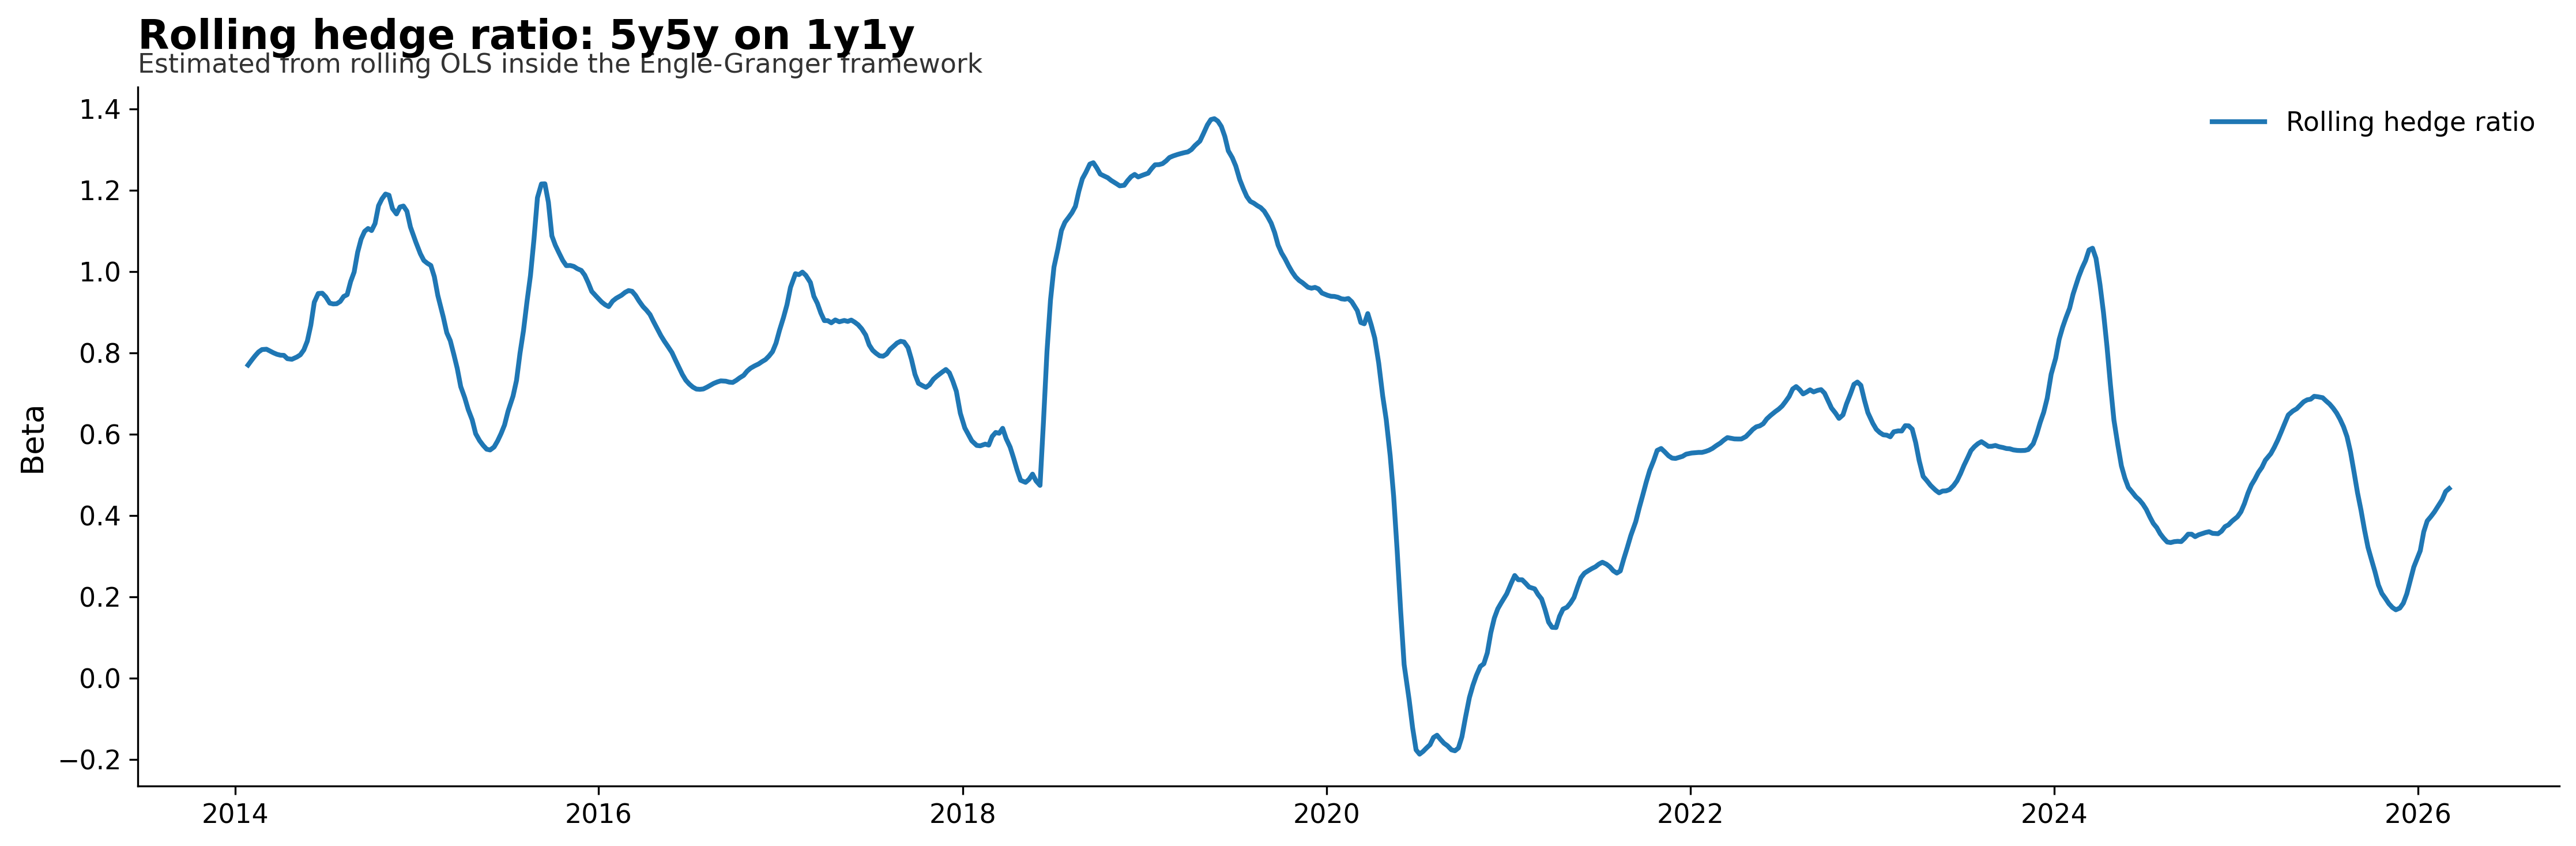
\includegraphics[width=0.92\textwidth]{figures/05_cointegration/fig_24_rolling_cointegration_beta.png}
		\caption{Rolling hedge ratio from the rolling OLS step inside the Engle--Granger cointegration framework.}
		\label{fig:rolling_coint_beta}
	\end{figure}
	
	\begin{figure}[H]
		\centering
		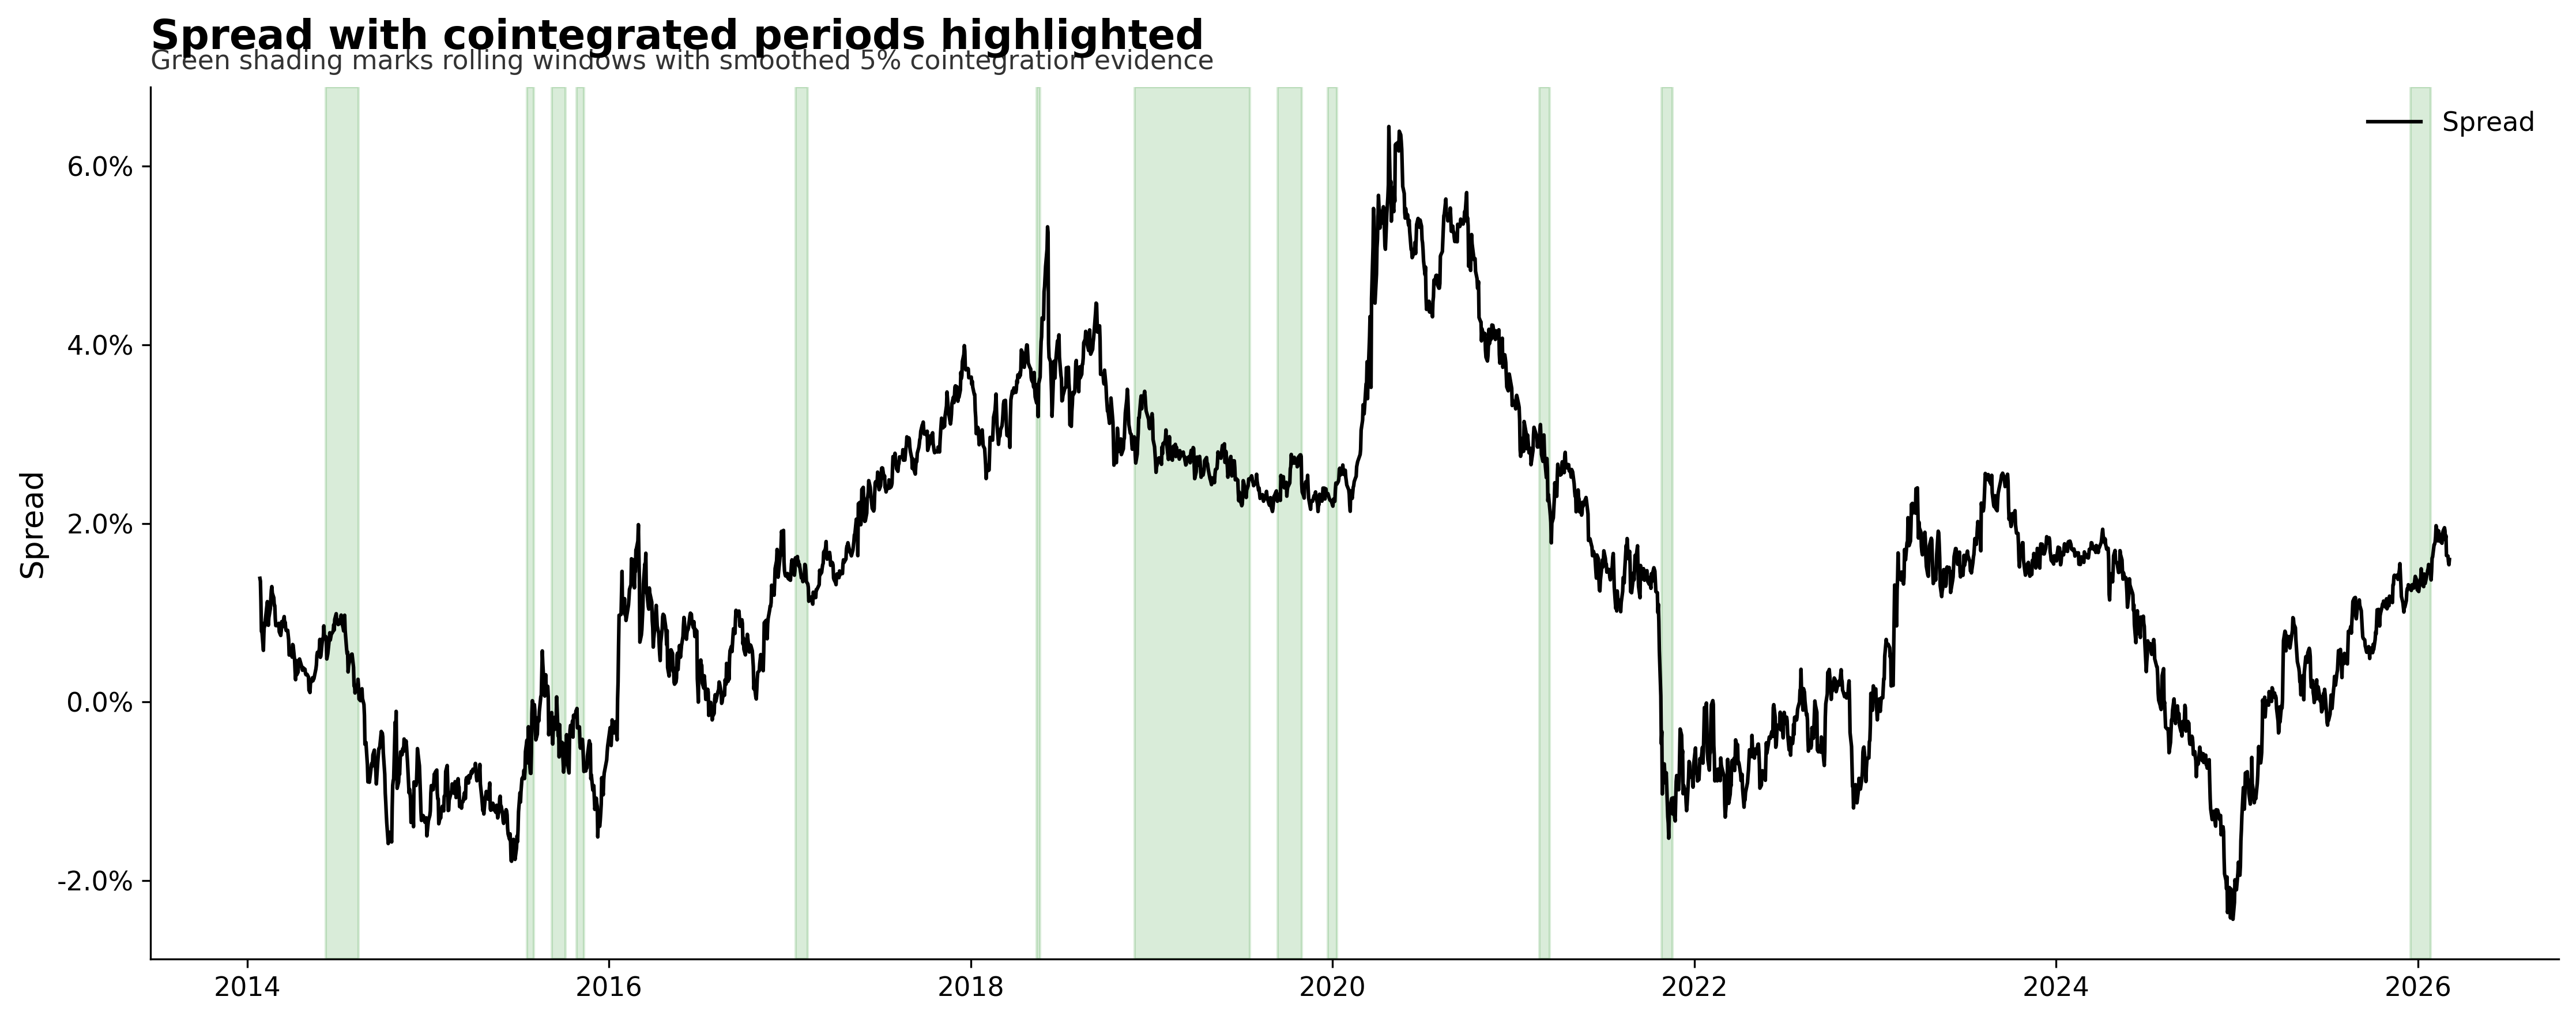
\includegraphics[width=0.92\textwidth]{figures/05_cointegration/fig_25_spread_with_cointegrated_periods.png}
		\caption{Observed spread with rolling windows classified as cointegrated highlighted in green.}
		\label{fig:spread_coint_periods}
	\end{figure}
	
	\begin{table}[H]
		\centering
		\footnotesize
		\begin{tabular}{rrrrrrrrrr}
			\toprule
			Window & Step & Pct. strong & Pct. moderate & Pct. weak & Pct. none & Avg beta & Beta std & Avg half-life & Median half-life \\
			\midrule
			252 & 5 & 0.0333 & 0.0965 & 0.0982 & 0.7720 & 0.6948 & 0.3317 & 30.15 & 17.31 \\
			\bottomrule
		\end{tabular}
		\caption{Summary statistics for the rolling cointegration analysis between \(5y5y\) and \(1y1y\).}
		\label{tab:rolling_coint_summary}
	\end{table}
	
	\begin{table}[H]
		\centering
		\footnotesize
		\begin{tabular}{lrrrrrrrr}
			\toprule
			Regime & Obs. & Total PnL & Annualized PnL & Annualized vol & Sharpe & Avg abs. pos. & Annual turnover & Hit ratio \\
			\midrule
			strong   & 100  & -86{,}384.81  & -217{,}689.72 & 1{,}029{,}976.00 & -0.21 & 0.76 & 2.52 & 0.40 \\
			moderate & 290  & -441{,}934.40 & -384{,}025.75 & 1{,}851{,}741.00 & -0.21 & 0.77 & 3.48 & 0.36 \\
			weak     & 292  & -865{,}951.30 & -747{,}327.80 & 1{,}507{,}185.00 & -0.50 & 0.68 & 11.22 & 0.34 \\
			none     & 2320 & 3{,}645{,}198.00 & 395{,}943.95 & 1{,}807{,}593.00 & 0.22 & 0.60 & 9.02 & 0.31 \\
			\bottomrule
		\end{tabular}
		\caption{Backtest performance grouped by rolling cointegration regime.}
		\label{tab:pnl_by_coint_regime}
	\end{table}
	
	\begin{table}[H]
		\centering
		\footnotesize
		\begin{tabular}{lrrrrrr}
			\toprule
			Regime & Obs. & Avg spread & Spread vol & Avg abs. daily change (bp) & Avg half-life & Avg beta \\
			\midrule
			strong   & 100  & 2.3840 & 0.6208 & 6.20 & 8.02  & 1.1701 \\
			moderate & 290  & 1.7287 & 1.2822 & 9.42 & 9.67  & 0.8953 \\
			weak     & 292  & 0.9326 & 1.4160 & 8.55 & 10.82 & 0.7215 \\
			none     & 2320 & 1.3276 & 1.8017 & 9.91 & 51.01 & 0.6462 \\
			\bottomrule
		\end{tabular}
		\caption{Spread statistics grouped by rolling cointegration regime.}
		\label{tab:spread_stats_coint_regime}
	\end{table}
	
\end{document}
